\chapter{Dynamical systems}
\label{h:dynamical}

\begin{quote}
The mathematician's patterns, like the painter's or the poet's must be beautiful; the ideas, like the colours or the words must fit together in a harmonious way. Beauty is the first test.

--- Godfrey H. Hardy
\end{quote}

\begin{quote}
As for everything else, so for a mathematical theory: beauty can be perceived but not explained.

--- Arthur Cayley
\end{quote}

\chaptertoc

In this chapter, we will study some aspects of the dynamics of nonlinear systems. We will see that these systems can exhibit wonderfully complex and intricate phenomena, producing both pretty pictures and profound insights into the behaviour of physical processes.

After an example from the photonics world, we will look at \textbf{1D discrete systems}, and study aspects like cobweb plots, fixed points and their stability, as well as periodic points. We'll look at how to visualise the properties of the family of logistic maps in a bifurcation diagram. We'll also define chaos as being the sensitive dependence on initial conditions.

\textbf{2D discrete systems} are studied next, and we'll introduce the concept of saddle points. After studying linear maps, we'll show how to locally approximate a nonlinear map by a linear one. We briefly discuss the importance of stable and unstable manifolds.

Finally, we will talk about \textbf{continuous systems}, i.e. systems that are described by differential equations instead of difference equations. We will show how to use phase portraits to represent their behaviour, and finish with the famous example of the Lorentz attractor.

\pagebreak

\sectionugent{Example: chaos in a photonic system}

\begin{marginfigure}
\centering
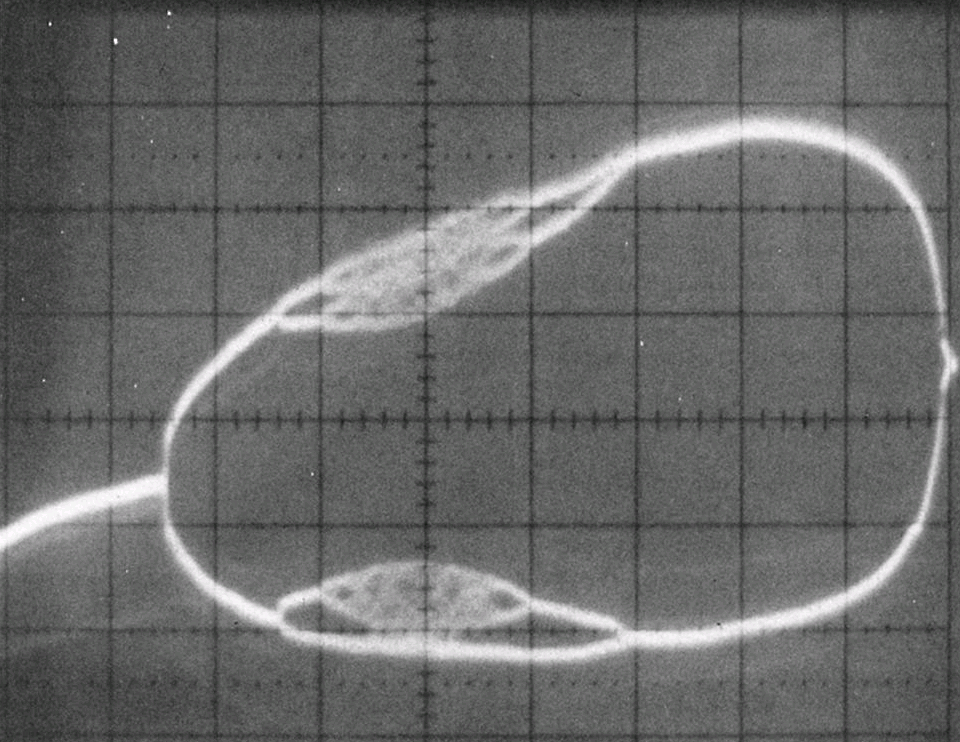
\includegraphics{dynamic/figures/CO2_chaos}
\caption{Sampled laser intensity as a function of the DC bias $A$ in a CO$_2$--laser.}
\label{fig-co2}
\end{marginfigure}

In 1991, scientists at the University of Lille studied a CO$_2$--laser which contained an electrooptic absorber inside the cavity to modulate the output intensity of the laser beam. An alternating current $I(t)=A+B \sin (\omega t)$ was applied to the modulator. The modulation amplitude $B$ was kept fixed at 3V, and the modulator frequency $\omega$ was set to 640 kHz, a resonance frequency of the laser. Next, the experimenters varied the DC bias $A$ from 60V to 460V and observed what happened to the laser output power $P(t)$. They sampled the output 640 000 times per second, i.e. in lockstep with the modulation frequency. They did this experiment for various values of the DC bias to produce the oscilloscope picture of Fig.~\ref{fig-co2}.

\begin{cue}
For low values of the DC bias, there is only a single branch. What does this mean for the time evolution of the laser intensity?
\end{cue}

\begin{marginfigure}
\centering
% -.5*sin(x)+0.9+.5*sin(0.5*x)
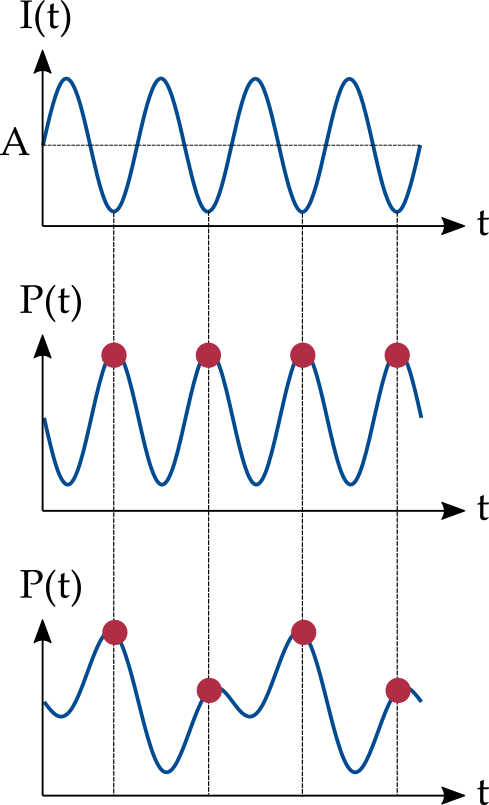
\includegraphics{dynamic/figures/lille}
\caption{Time evolution of the modulator current (top), of the laser output for low DC bias (middle) and of the laser output for higher DC bias.}
\label{fig-lille}
\end{marginfigure}

For low values of the DC bias, for every bias value there is only a single value when sampling once per period. This means that the laser intensity varies with the same frequency as the modulation current, which is just what you would expect for a linear system (Fig. \ref{fig-lille} middle).

\begin{cue}
For larger DC bias, there are suddenly two branches in the curves. What can you say now about the time evolution?
\end{cue}

These two branches in the curves mean that e.g. for odd periods you get a certain sample value, whereas for even periods you get a different value. This means that the laser oscillation takes two periods of the modulation to repeat. This pattern with doubled period is called a \textbf{subharmonic} of the modulation period (Fig. \ref{fig-lille} bottom).

Increasing the DC bias even further leads to patterns which take 4, 8 or more modulation periods to repeat. There is even a certain range where the laser output varies between so many levels that it looks very chaotic.

The combination of CO$_2$--laser plus absorber can be described by a set of relatively simple nonlinear rate equations (see e.g. the course 'High speed photonic components'). At first sight, it is very surprising that dynamical systems which are described by relatively simple--looking differential equations can exhibit such rich behaviour.

In this chapter, we will study some aspects of this complex behaviour of dynamical systems, starting from very simple 1D models described by difference equations. Higher dimensional systems and systems described by differential equations instead of difference equations will also be treated.


\sectionugent{Dynamical systems}

A \textbf{dynamical system} consists of a set of possible states, together with a rule that determines the present state in terms of the past states. E.g., a simple model for growth of bacteria in a lab culture is that the population doubles each hour.

\begin{cue}
  What would the update rule of such a system look like?
\end{cue}

The update rule of this system is

\begin{equation}
x_n = f(x_{n-1}) = 2 x_{n-1} \label{eq-exp-growth}
\end{equation}

here, the state $x$ designates the population size, and the subscript $n$ stands for the state at time step $n$, in this case the state after $n$ hours.  

Based on the properties of the update rule, we can distinguish several types of dynamical systems.

In this chapter, we require the rule to be \textbf{deterministic}, which means we can determine the present state uniquely from the past states. If we also consider randomness, e.g. in the presence of noise, our system is \textbf{stochastic}.

If the update rule is applied at discrete times, the system is called a \textbf{discrete--time} system. In the limit of infinitesimally small time steps, the governing rules become a set of differential equations, and we end up with a \textbf{continuous--time} system.

\pagebreak

\sectionugent{1D maps - logistic growth}

A function $f$ whose input and output space are the same is called a \textbf{map}. The evolution of a dynamical system is governed by multiple applications of the update rule $f$. Let us define $f^2(x)=f(f(x))$ and more generally define $f^k(x)$ as the results of applying $f$ to $x$ $k$ times. The set of points ${x_0, f(x_0), f^2(x_0), ...}$ is called the \textbf{orbit} of $x_0$ under $f$. The starting point $x_0$ is called the \textbf{initial value} of the orbit.

Of interest in the study of dynamical systems is the limiting behaviour of $f^k(x)$ for large values of $k$. For the exponential growth scenario of Eq.~\ref{eq-exp-growth}, the population will clearly increase without bound, which is obviously not a realistic model.

Let's build a slightly more realistic model, where e.g. competition for scarse resources will put brakes on growth as soon as the population gets too large.. First of all, rather than working with integer population values, we switch to a population size which is normalised between 0 and 1, with 1 representing some kind of reference value.

\begin{cue}
Instead of having a multiplication by 2 every time step, can you propose a simple model where this factor reduces the larger the population gets? 
\end{cue}

If we replace e.g. 2 by $2(1-x)$, we see that this factor is still close to 2 for low values of $x$, but reduces to 0 as $x$ starts approaching 1.

The whole update rule then becomes

\begin{equation}
f(x) = 2 x (1-x) \label{eq-logistic-growth}
\end{equation} 

Contrary to the exponential growth model, this so--called \textbf{logistic growth} model has a nonlinear update rule.

\begin{exer}
% difficulty: trivial
Show using computer simulations that populations evolving under the rule $f(x) = 2 x (1-x)$ tend to the population of 0.5 as time evolves. Do this for several initial values. You will find that the size $x=0.5$ eventually 'attracts' any of these starting populations.
\end{exer}

\pagebreak

\sectionugent{Cobweb plots}

A cobweb plot is a graphical representation of the orbit of an initial value under a 1D map. It is obtained by drawing the graph of the update rule, together with the diagonal $y=x$ (see Fig.~\ref{fig-cobweb1}).

\begin{marginfigure}
\centering
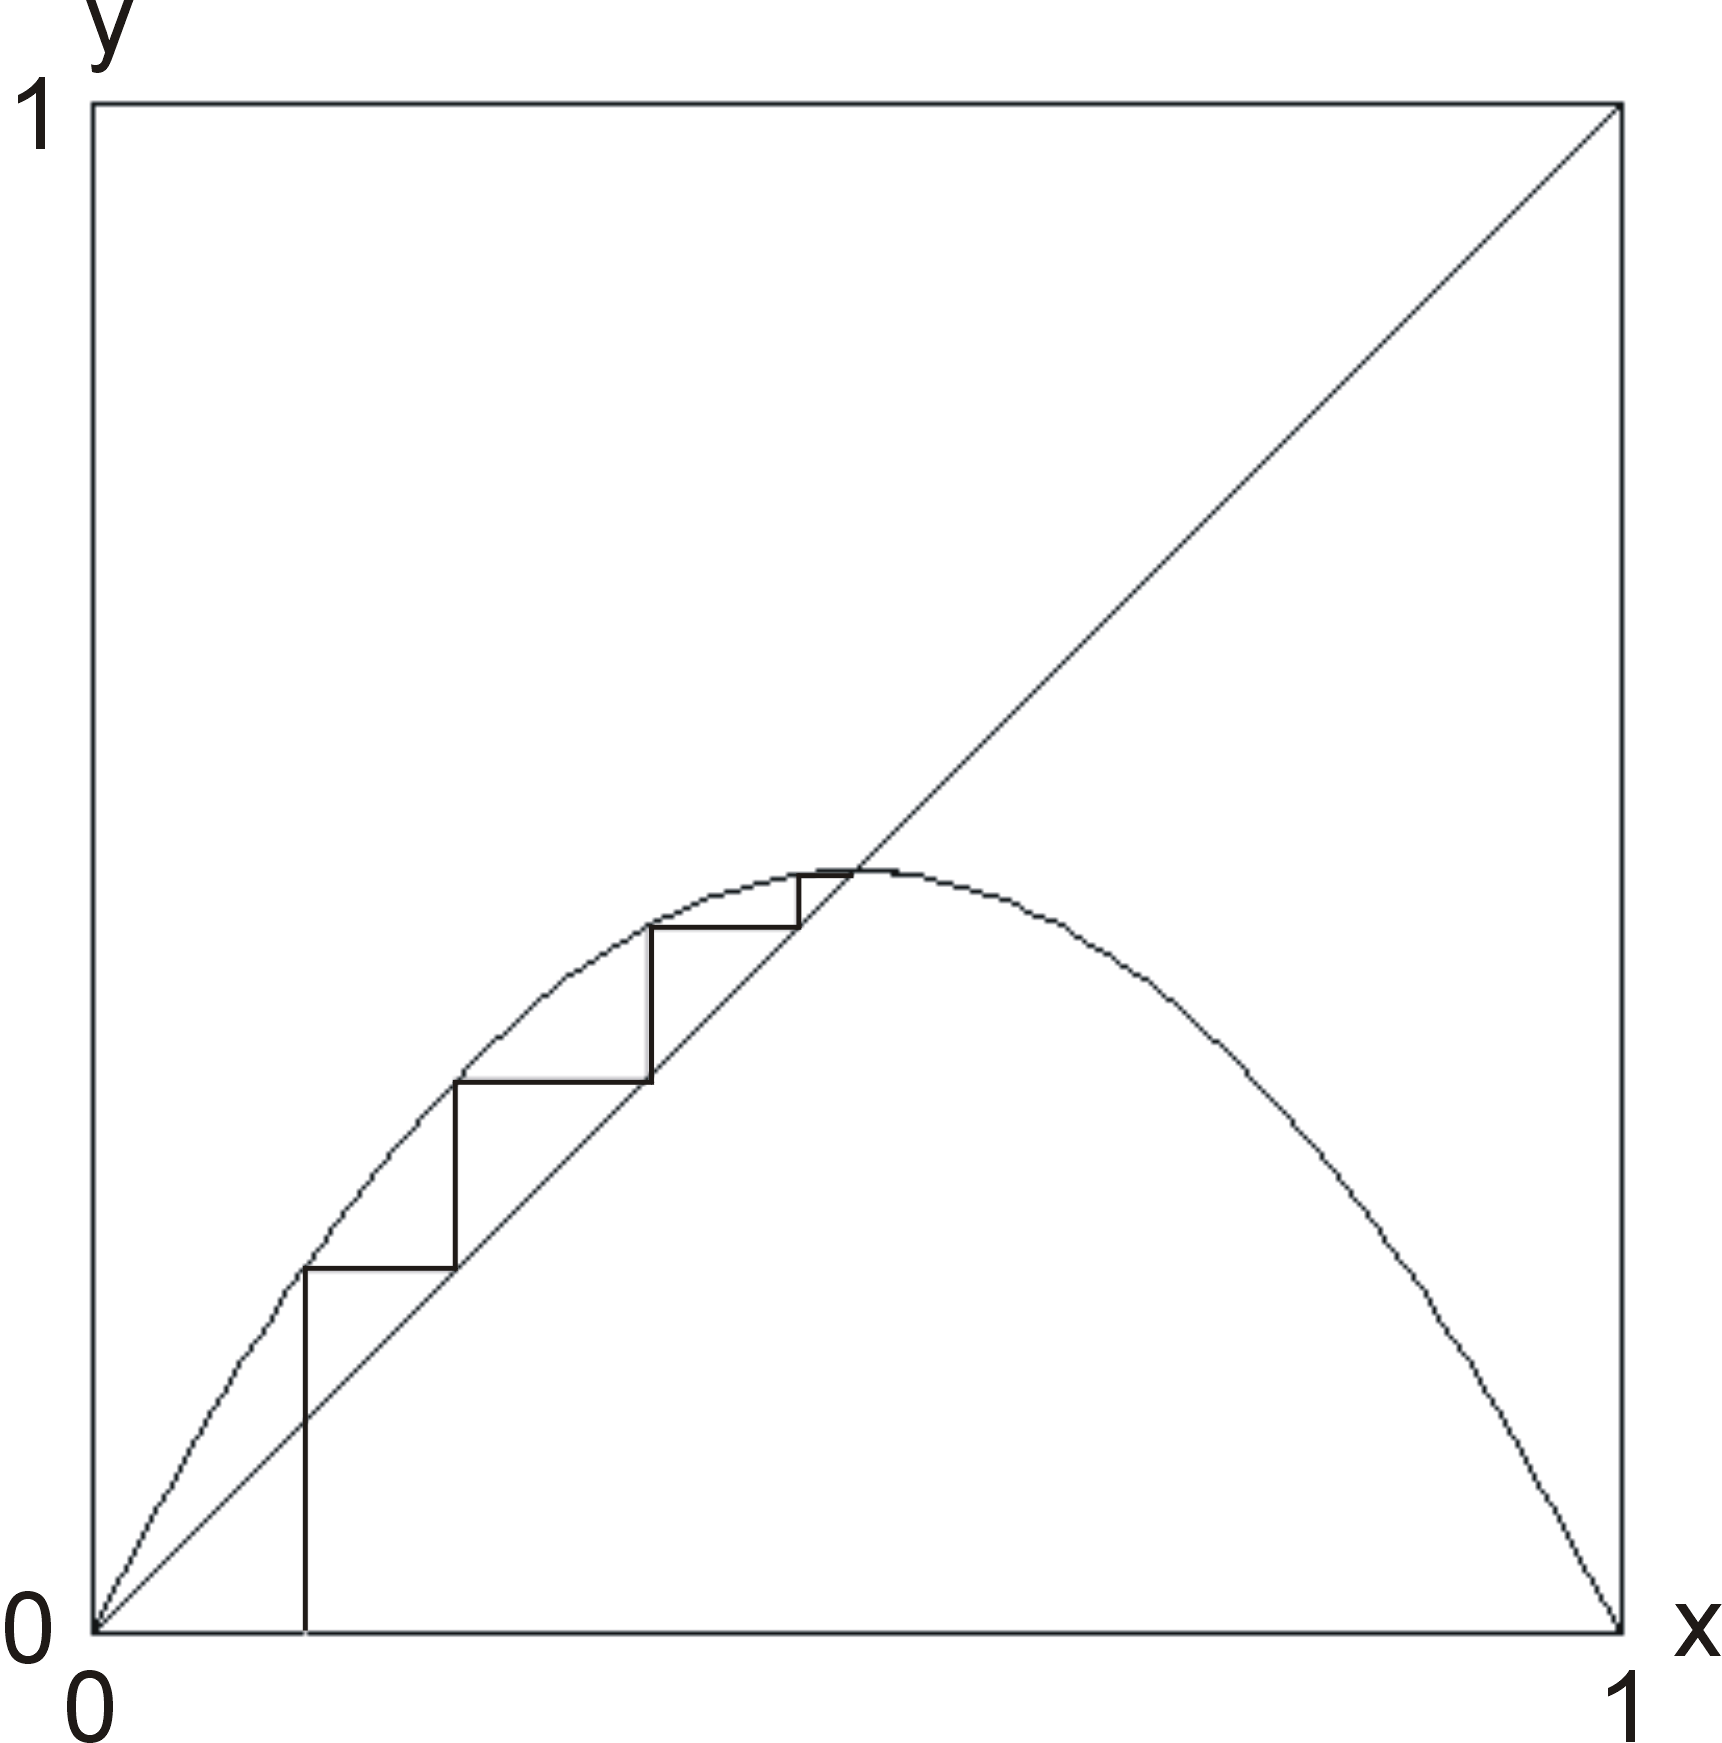
\includegraphics{dynamic/figures/cobweb1}
\caption{Cobweb plot for $f(x)=2x(1-x)$.}
\label{fig-cobweb1}
\end{marginfigure} 

\begin{cue}
Study this figure and convince yourself that this indeed represents an orbit. More specifically, explain why and when you use horizontal vs vertical lines, and whether they stop at the update rule or at the line under 45 degrees. Also, why is it important that this straight line has an angle of 45 degrees?
\end{cue}

Sketching the orbit of an initial point is done as follows. E.g., starting with the input value $x_0=0.1$ and $f(x)=2x(1-x)$ in Fig.~\ref{fig-cobweb1}, we can easily plot $f(0.1)$ by drawing a vertical line starting from $x_0=0.1$ to the curve $f(x)$, which gives us a value of $0.18$. Next, we need to turn this output value of $0.18$ to an input value to compute $f(0.18)$. This is done by drawing a horizontal line from the input--output pair $(0.1,0.18)$ until it reaches the diagonal $y=x$. Now, the process can be repeated by drawing a sequence of vertical and horizontal line segments between the curve of the update rule and the diagonal.

From the cobweb plot, it is clear that the orbit will converge to the point $x=0.5$, which lies on the intersection of the graph of the update function and the diagonal.

Such points where $f(x)=x$ are called \textbf{fixed points}. They are of extreme importance when studying the dynamics of a system, as they contain information on the asymptotic behaviour of the system.

\begin{exer}
% difficulty: normal
% ugent
Let $f$ be the map given by $f(x) = (3x-x^3)/2$. Draw cobweb plots for orbits with initial values $x=1.6$ and $x=1.8$ (Fig. \ref{fig-cobweb-ex}). Calculate the fixed points of this map. What happens with orbits starting out in the vicinity of each of these fixed points?
\end{exer}

\begin{figure}
\centering
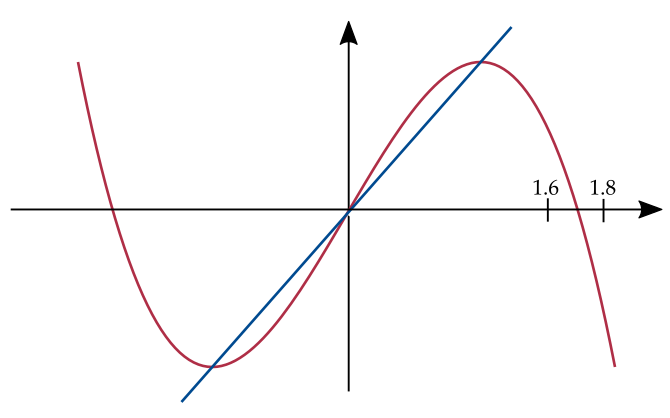
\includegraphics{dynamic/figures/cobweb_ex}
\caption{For $f(x) = (3x-x^3)/2$, draw cobweb plots for orbits with initial values $x=1.6$ and $x=1.8$.}
\label{fig-cobweb-ex}
\end{figure} 


\pagebreak

\sectionugent{Sinks and sources}

Not all fixed points are alike. A \textbf{stable} fixed point has the property that points near it will move even closer to it as the dynamical system evolves. For an \textbf{unstable} fixed point, the opposite is true: points starting out in its neighbourhood will rapidly move away as time progresses.

A good analogy is that a ball at the bottom of a valley is stable, while a ball balanced at the tip of mountain will be unstable.

Stability is an important concept as real--world systems are constantly subjected to small perturbations. Therefore, a steady state observed in a real system must correspond to a stable fixed point. If the fixed point were unstable, small perturbations would move the orbit away from the fixed point, which would then be not observed.

A stable, attracting fixed point is often called a \textbf{sink}, while an unstable, repelling fixed point is called a \textbf{source}.

To formulate this more precisely, let's first introduce the concept of an \textbf{epsilon neighbourhood} $N_\epsilon(p)$, which is the set of all real numbers within a distance $\epsilon$ of $p$:

\begin{equation}
N_\epsilon(p) = \{x \in \mathbb{R} ; |x-p| < \epsilon\}
\end{equation} 

\begin{cue}
Try and come up with a definition of a sink. How does the epsilon neighbourhood come into play? 
\end{cue}

\begin{marginfigure}
\centering
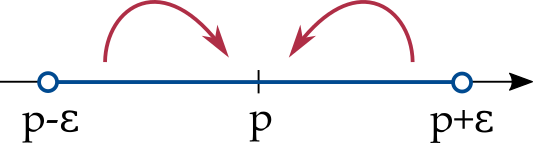
\includegraphics{dynamic/figures/sink}
\caption{All points in the neigbourhood of a sink $p$ eventually end up at $p$ after applying the map.}
\label{fig-sink}
\end{marginfigure}

We need to account for the fact that in general, only points that are 'close enough' to the sink will eventually end up there. So, we can say that a fixed point is a sink if there exists an $\epsilon > 0$ such that for all points $x$ in the epsilon neighbourhood the map will eventually take that point to fixed point $p$.

Or, in symbols:

\begin{equation}
\exists \, \epsilon : \forall x \in  N_\epsilon(p) : \lim_{k \to \infty} f^k(x) = p
\end{equation}

\begin{marginfigure}
\centering
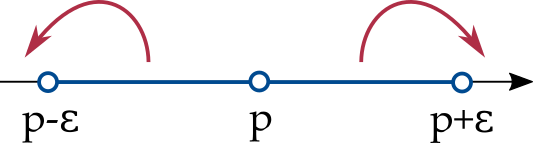
\includegraphics{dynamic/figures/source}
\caption{All points in the neigbourhood of a sink $p$ (except for $p$ itself) eventually end up outside of that neighbourhood after applying the map.}
\label{fig-source}
\end{marginfigure}

Similarly, a fixed point is called a source if there exists an epsilon neighbourhood $N_\epsilon(p)$ such that each $x$ in $N_\epsilon(p)$ except $p$ eventually maps outside of $N_\epsilon(p)$:

\begin{equation}
\exists \, \epsilon : \forall x \in  N_\epsilon(p) \setminus \{p\} : \exists \, K : \forall k > K : f^k(x) \notin  N_\epsilon(p)
\end{equation}

\begin{cue}
Why do we need to exclude $p$ from this definition?
\end{cue}

Since $p$ is a fixed point, it will always map to itself, rather than running away outside of the epsilon neighbourhood.

\begin{cue}
Why don't we say for the definition of the source simply that $\lim_{k \to \infty} f^k(x) \ne p$, in analogy with the definition of the sink?
\end{cue}

For the source, we cannot use the limit of the orbit in the definition, for the simple reason that perhaps this limit is not defined! Indeed, later we'll see plenty of examples where orbits do not settle. Therefore, we demand instead that the orbit leaves the epsilon neighbourhood.

\pagebreak

\sectionugent{Stability theorem for fixed points}

Next question: how can we determine from the shape of $f$ whether a fixed point is a source or a sink? The answer lies in the following theorem:

Let $f$ be a smooth map of $\mathbb{R}$ with fixed point $p$. 
\begin{enumerate}
\item
If $|f'(p)| < 1$, then $p$ is a sink.
\item 
If $|f'(p)| > 1$, then $p$ is a source. 
\end{enumerate}

We only prove the first part, as the second is very similar.

\begin{cue}
Since the theorem involves derivatives, write down $|f'(p)|$ as a limit involving a neighbouring point $x$.  
\end{cue}

From the definition of the derivative, we get (for points $x \ne p$)

\begin{equation}
\lim_{x \to p} \frac{\left|f(x)-f(p)\right|}{|x-p|} = \left|f'(p)\right|
\end{equation} 

Since $|f'(p)| < 1$, you can always squeeze in an extra number $a$ between $|f'(p)|$ and 1.

\begin{cue}
Consider $\frac{\left|f(x)-f(p)\right|}{|x-p|}$ as a new function $g(x)$, for which we know the value at $x=p$. What can you say about the values of $g(x)$ for points close to $x=p$?  
\end{cue}

\begin{marginfigure}
\centering
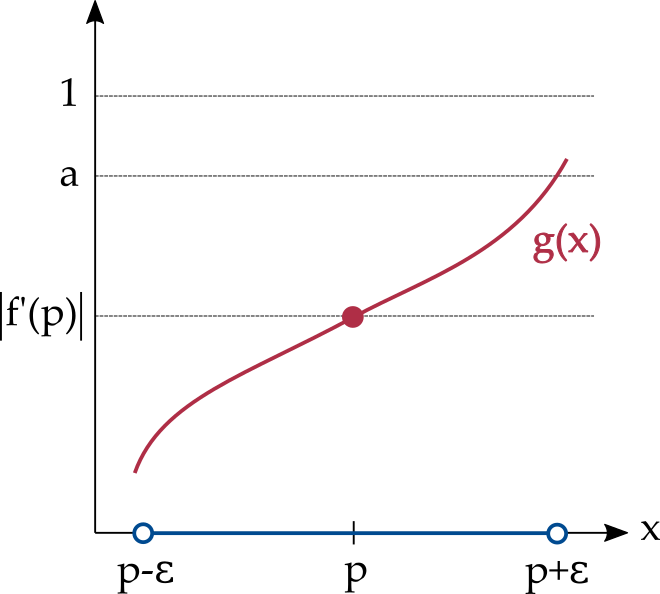
\includegraphics{dynamic/figures/stab}
\caption{Epsilon neighbourhood used in the proof of the stability theorem.}
\label{fig-eps-stab}
\end{marginfigure}

Assuming continuous functions, this means that there must be a neighbourhood $N_\epsilon(p)$ where (see Fig. \ref{fig-eps-stab})

\begin{equation}
\frac{\left|f(x)-f(p)\right|}{|x-p|} < a, \hspace{.5cm} \forall x \in N_\epsilon(p)
\end{equation}

\begin{cue}
Will $f(x)$ also be in $N_\epsilon(p)$ or not? Don't forget that $p$ is a fixed point. 
\end{cue}

Using the fact that $p$ is a fixed point, we get

\begin{equation}
\left|f(x)-p\right| < a |x-p|,  \hspace{.5cm} \forall x \in N_\epsilon(p) \label{eq-stab-fix}
\end{equation}

So, $f(x)$ is closer to $p$ than $x$ was to $p$ by at least a factor of $a$, meaning that $f(x)$ is also in $N_\epsilon(p)$.

Let's rewrite Eq.~\ref{eq-stab-fix} slightly:

\begin{equation}
\left|f^1(x)-p\right| < a \left|f^0(x)-p\right|,  \hspace{.5cm} \forall x \in N_\epsilon(p)
\end{equation} 

\begin{cue}
Why can we apply this procedure again? Do so!  
\end{cue}

Since $f^1(x)$ is also in $N_\epsilon(p)$, we can repeat the above procedure to get

\begin{equation}
\left|f^k(x)-p\right| < a\left|f^{k-1}(x)-p\right| < a^2\left|f^{k-2}(x)-p\right|< ... < a^k |x-p| 
\end{equation}  

\begin{cue}
Finally, take the limit of $k \to \infty$. Why did we need to introduce the variable $a$?
\end{cue}

Since $a<1$, we get eventually that

\begin{equation}
\lim_{k \to \infty} \left|f^k(x)-p\right| = 0
\end{equation} 

This proves that $p$ is a sink.

The set of initial conditions that is attracted to the sink is called the \textbf{basin} of the sink. From the proof of the stability theorem, we get that the basin of a sink contains at least a small epsilon neighbourhood, but in practice sinks often attract a large set of initial conditions.

Finally, note that the stability theorem does not say anything about the case $|f'(p)|=1$.

\begin{exer}
% difficulty: trivial
% ugent
Discuss the stability of the fixed points of the map $f(x) = (3x-x^3)/2$.
\end{exer}

\begin{exer}
% difficulty: normal
Discuss the stability of the fixed points of the map $f(x) = x^3 + x$.
\end{exer}

\begin{exer}
% difficulty: normal
Prove the stability theorem explicitly for the case of a source.
\end{exer}

\pagebreak

\sectionugent{Periodic points}

\begin{marginfigure}
\centering
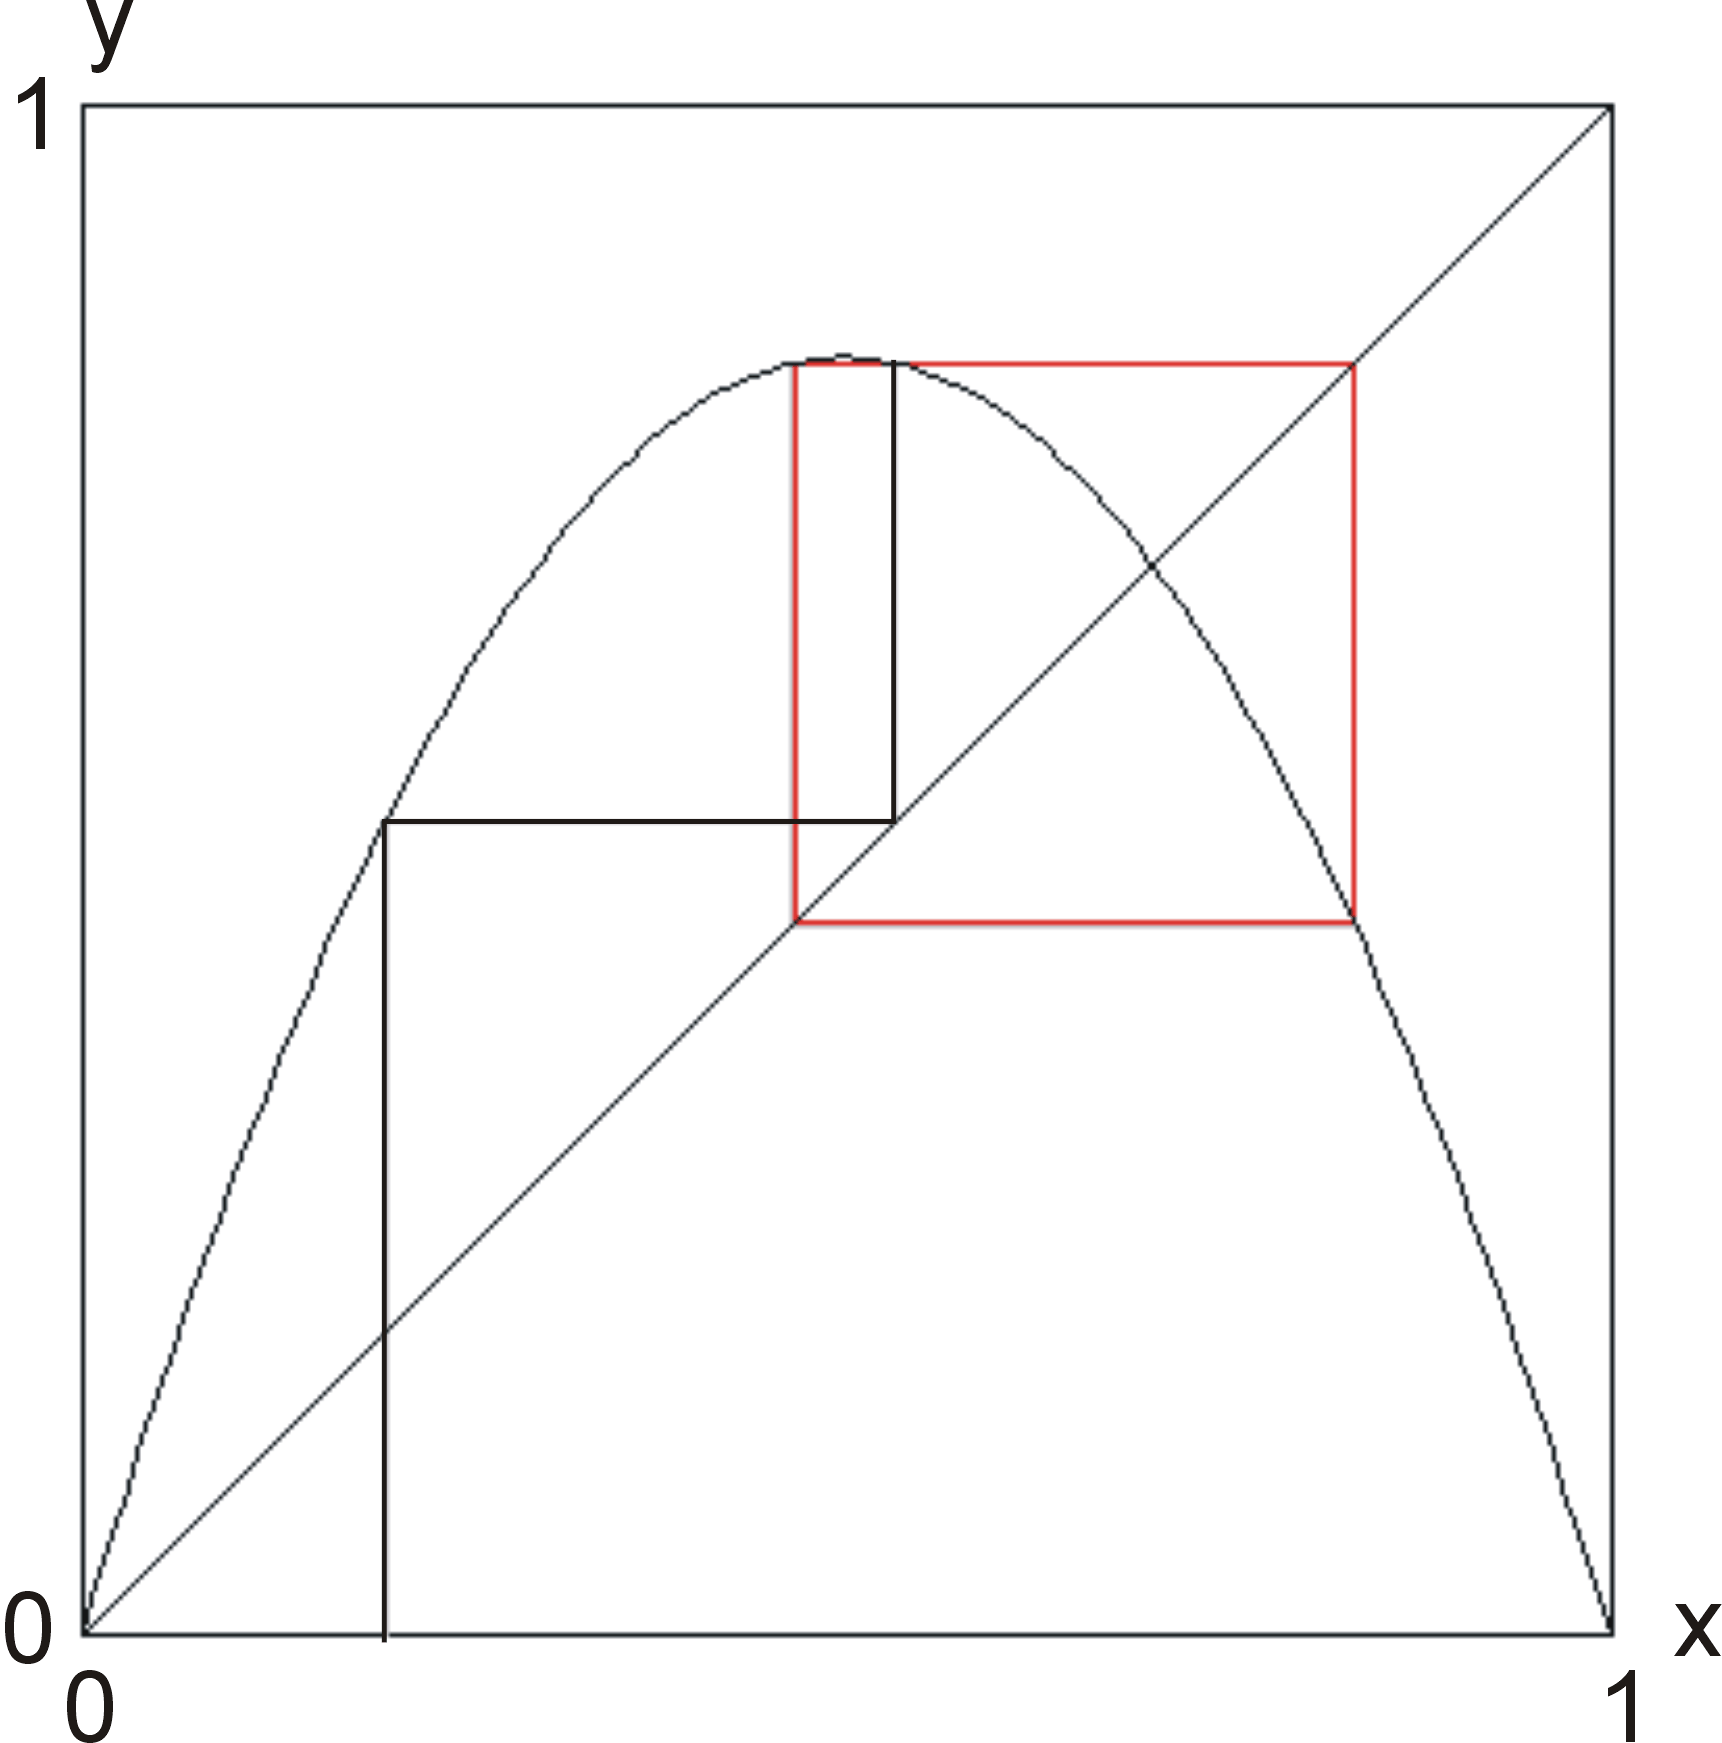
\includegraphics{dynamic/figures/cobweb2}
\caption{Cobweb plot for $f(x)=3.3x(1-x)$.}
\label{fig-cobweb2}
\end{marginfigure}

If we change the proportionality constant $a$ of the logistic map $f_a(x)=ax(1-x)$ to 3.3, we get a different behaviour than what we have seen so far. The fixed points are $x=0$ and $x=23/33$, both of which are unstable. So, without any fixed points to attract them, where do the orbits go? Using a calculator or a computer, it is easy to show that the orbit settles into a pair of alternating values $p_1=0.4794$ and $p_2=0.8236$. Fig.~\ref{fig-cobweb2} plots the cobweb diagram for this case.

\begin{cue}
Note that $f(p_1)=p_2$ and $f(p_2)=p_1$. What does that mean in terms of $f^2$, i.e. $f$ applied twice?
\end{cue}

Another way of looking at this it saying that $f^2(p_1)=p_1$, so $p_1$ is a fixed point of $h=f^2$ (the same is obviously true for $p_2$).

More formally, we call $p$ a \textbf{periodic point of period $\mathbf k$} (or period--$k$ point) of a map $f$ if $f^k(p)=p$ and $k$ is the smallest positive integer for which this is true. E.g., a fixed point of $f^2$ will trivially also be periodic with periods 4,6,8, ... , but we only focus on the smallest of these numbers.

Just like fixed points, period--$k$ orbits can be attracting (sinks) or repelling (sources).

\begin{cue}
Since a period--$k$ point is a fixed point of $f^k$, apply the stability theorem to the map $f^k$,
\end{cue}

For a period--2 point, we need to evaluate $|f^2(p_1)|$, which can be done easily with the chain rule:

\begin{equation}
|f^{2'}(p_1)| = |f'(f(p_1)) f'(p_1)| = |f'(p_2) f'(p_1)|
\end{equation}  

This can be easily generalised to period--$k$ points:

\begin{exer}
% difficulty: trivial
% ugent  
Show that the following holds: a periodic orbit $\{p_1, p_2, ..., p_k\}$ is a sink if

$$|f'(p_1) f'(p_2) ... f'(p_k)| < 1$$

and a source if

$$|f'(p_1) f'(p_2) ... f'(p_k)| > 1$$

\end{exer}


Note that stability is a collective property of the periodic orbit, in the sense that $f^{k'}(p_i) = f^{k'}(p_j)$ for all values of $i$ and $j$.

\begin{exer}
% difficulty: trivial
Is any fixed point of $f^k$ a period--$k$ point of $f$?
\begin{sol}
No, there might be a smaller integer $n$ for which $f^n(p)=p$.  
\end{sol}
\end{exer}

\begin{exer}
% difficulty: normal
% credits: Chaos - Alligood T1.5
Verify that the map $f(x)=2x^2-5x$ has fixed points at 0 at 3. Use this information to more easily find a period-2 orbit for $f$, without needing to solve for the zeroes of a fourth-order polynomial.
\end{exer}


\pagebreak

\sectionugent{The family of logistic maps}

We have already seen that the scaling parameter $a$ in the family of logistic maps $f_a(x)=ax(1-x)$ can have a large influence on the behaviour of the system: for some ranges of $a$ there is only one attracting solution, for other ranges there is a stable period--2 orbit. Although these cobweb diagrams can be pretty to look at, it would be nice to have a more compact snapshot containing the entire family of logistic maps.

\begin{figure}[H]
\centering
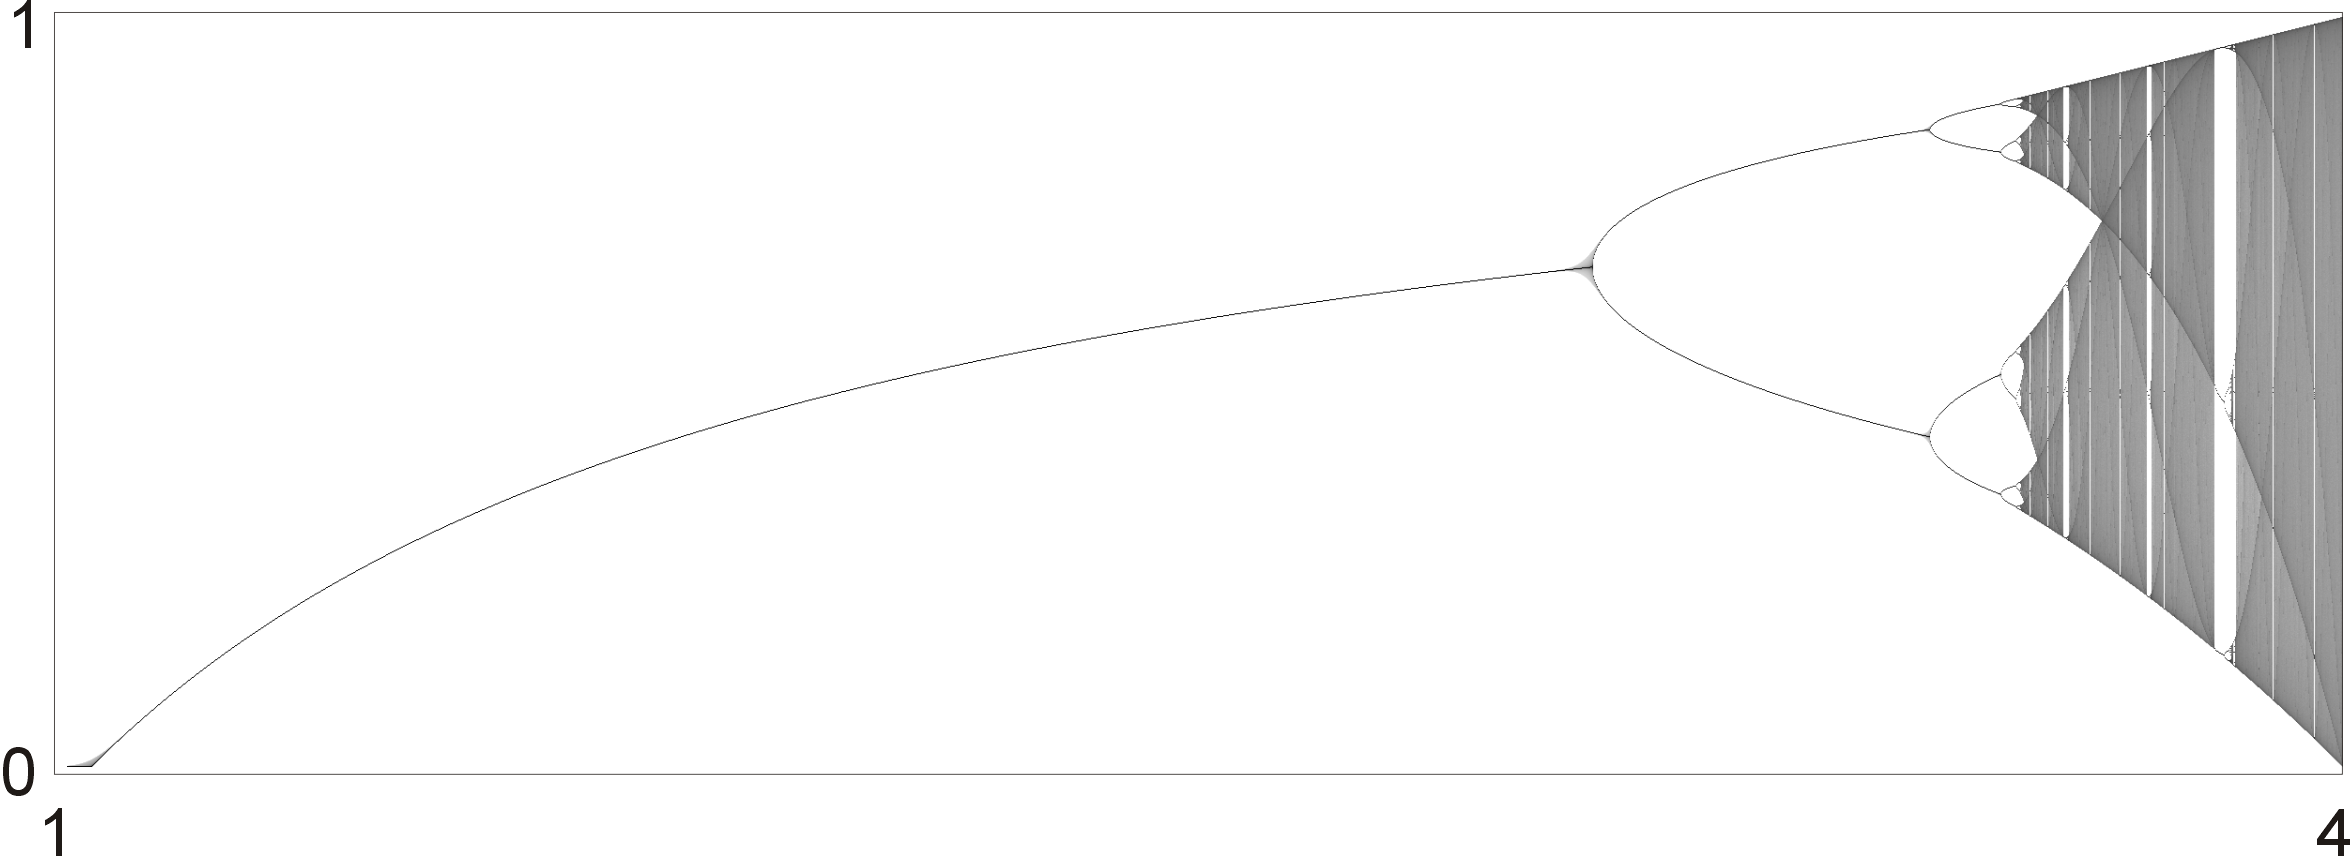
\includegraphics[width=10cm]{dynamic/figures/bifurcation}
\caption{Bifurcation diagram for the family of logistic maps for $f(x)=ax(1-x)$.}
\label{fig-bifur}
\end{figure} 

To visualise the behaviour of logistic maps for various values of $a$, we can make a diagram like the one in Fig.~\ref{fig-bifur}. On the horizontal axis we plot $a$, while the vertical axis shows $x$--values. The figure is constructed as follows: for each $a$--value, pick a random starting value $x$, and calculate its orbit under the map $f_a(x)$.

\begin{cue}
Should you plot all the points of the orbit in order to get Fig.~\ref{fig-bifur}?  
\end{cue}

Since we are only interested in the limiting behaviour and not the transient, discard e.g. the first 100 points of this orbit, and plot the remaining points of the orbit. Then increment $a$ and start the procedure again. The points that are plotted will (within the resolution of the picture) approximate either fixed or periodic sinks or other attracting orbits of the dynamic system.

One might ask how Fig.~\ref{fig-bifur} will change if different starting values of $x$ were selected. Surprisingly, it turns out that for the logistic map, nothing will change.

\begin{cue}
What does that statement tell you about the number of orbits for each value of $a$?  
\end{cue}

This indicates that for each $a$ value, there is at most one attracting orbit.

Fig.~\ref{fig-bifur} (and also Fig.~\ref{fig-co2}) is called a \textbf{bifurcation diagram} and shows the birth, evolution and death of attracting orbits. The term 'bifurcation' is used to describe significant changes in the set of attractors in a dynamical system. E.g. at $a=3$, there is a transition between a single sink and the emergence of a period--2 point. This type of bifurcation is called a \textbf{period--doubling bifurcation} or also (because of its characteristic shape) a \textbf{pitchfork bifurcation}. For $a$ slightly larger than 3.45, there appears to be a period--4 sink. In fact, there is an entire sequence of periodic sinks, one for each period 2, 4, 8, 16, 32,... . Such a sequence is called a \textbf{period--doubling cascade}.


\begin{exer}
Write a computer program that finds the $a$--values at which the bifurcations occur in the period--doubling cascade 2, 4, 8, 16, ... . Call the sequence of these values $a_n$, and calculate

$$\frac{a_{n-1} - a_{n-2}}{a_{n} - a_{n-1}}$$

What do you observe as $n$ tends towards infinity? Repeat the experiment for the period--3 cascade: 3, 6, 12,... . Also experiment with a different nonlinear map, like $f_a(x)=a-x^2$.

The number 4.669201609 is called \textbf{Feigenbaum's constant}.
\end{exer}

\begin{marginfigure}[-10cm]
% credits: Rockefeller University
% url: https://www.rockefeller.edu/news/26289-mitchell-feigenbaum-physicist-pioneered-chaos-theory-died/
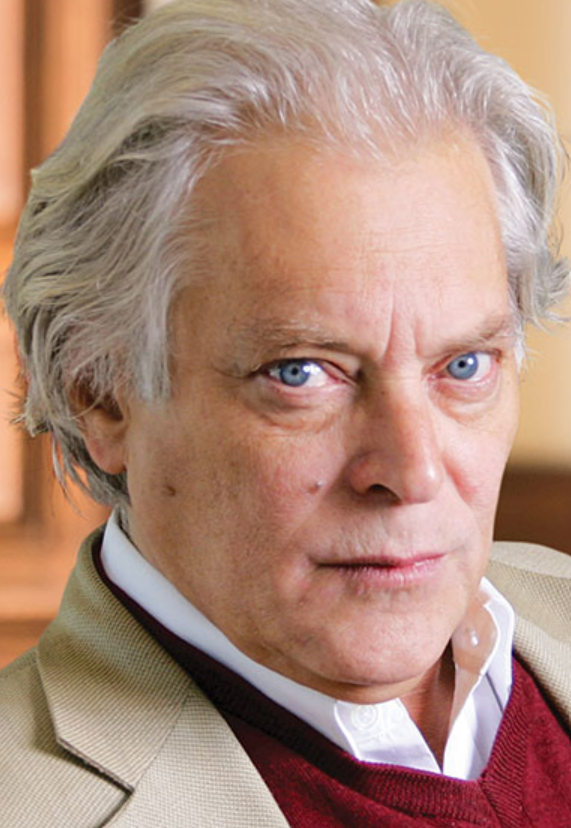
\includegraphics{dynamic/figures/m_feigenbaum}
\caption{Mitchell Feigenbaum (1944-2019)}
\end{marginfigure}

\begin{marginfigure}[-0.1cm]
\centering
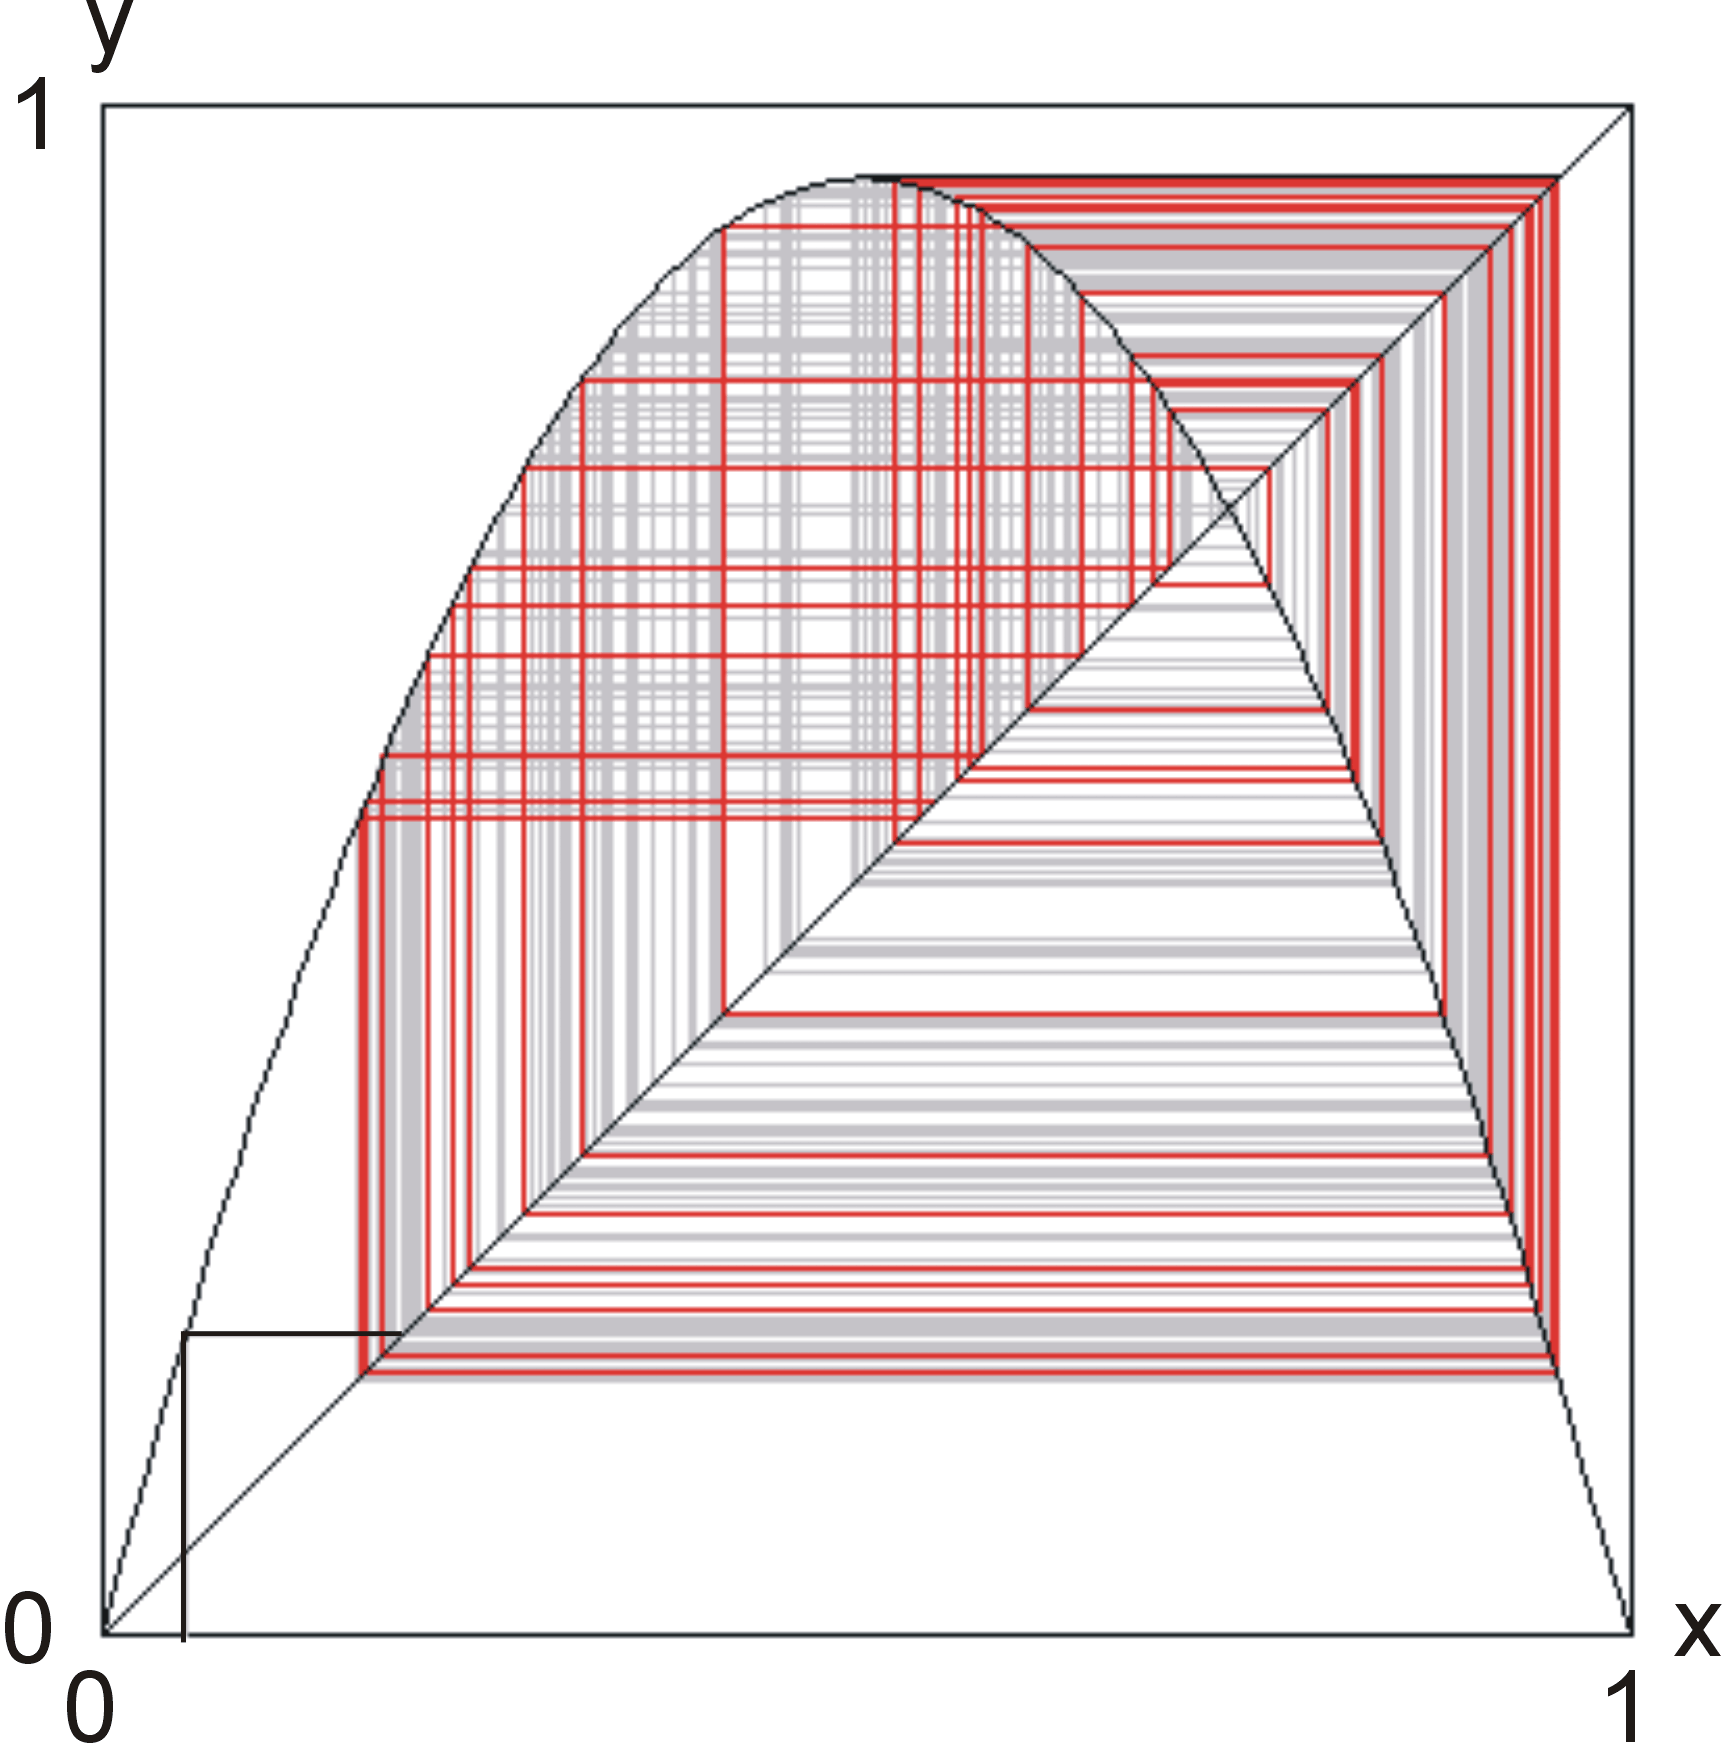
\includegraphics{dynamic/figures/cobweb3}
\caption{Cobweb plot for the logistic map in the case of a chaotic attractor.}
\label{fig-cobweb3}
\end{marginfigure}

For other values of the parameter $a$, the orbit appears to randomly fill out the interval $[0,1]$, or a subinterval. A typical cobweb plot for such a situation is shown in Fig.~\ref{fig-cobweb3}. These non--periodic attracting sets are called \textbf{chaotic attractors} and are obviously much harder to describe than periodic sinks.


So are these non--periodic attractors what we mean by 'chaos'? Partly. Another important concept in that regard is the sensitive dependence on initial conditions, which we will explore next.

\pagebreak

\sectionugent{Sensitive dependence on initial conditions}

\begin{table}[H]
\centering
\begin{tabular}{|c|c|c|}
\hline
${\mathbf n}$  & ${\mathbf f_n(0.3)}$ & ${\mathbf f_n(0.301)}$  \\
\hline
0  & 0.3000 & 0.3010  \\
\hline
1  & 0.8400 & 0.8416 \\
\hline
2  & 0.5376 & 0.5332 \\
\hline
3  & 0.9943 & 0.9956 \\
\hline
4  & 0.0225 & 0.0176 \\
\hline
5  & 0.0879 & 0.0692 \\
\hline
6  & 0.3208 & 0.2576 \\
\hline
7  & 0.8716 & 0.7650 \\
\hline
8  & 0.4476 & 0.7190 \\
\hline
9 & 0.9890 & 0.8081 \\
\hline
10 & 0.0434 & 0.6202 \\
\hline
\end{tabular}
\caption{Comparison of orbits of nearly identical points under the map $f(x)=4x(1-x)$.}
\label{table-sens}
\end{table}

Table~\ref{table-sens} shows the orbits of two points 0.3000 and 0.3010 under the map $f(x)=4x(1-x)$. Although these points start out close together, they quickly diverge. In fact, no matter how close together we choose these two points, they will eventually move apart. This sensitive dependence on initial conditions has some far--reaching implications. If a dynamic system exhibits these chaotic properties, it means we can never hope to accurately predict the long--term behaviour of the system \emph{in practice}, even though it is governed by deterministic and well--known rules. Sensitive dependence on initial conditions means that small variations in the initial state of the system (e.g. due to measurement errors or finite numerical precision), will always get amplified to such a degree that it is impossible to make long--term predictions on the evolution of the system. This is the hallmark of \textbf{chaos}.

To quantify how sensitive an orbit is to variations in initial conditions, we will now introduce the concept of Lyapunov numbers and Lyapunov exponents.

We already learnt that for fixed points, stability is heavily influenced by the derivative of the map. Also here, derivatives will play an important role.

\begin{cue}
Make a first-order approximation of $f(x)$ around a point $x_0$, and plug in for $x$ two neigbouring points $x_a$ and $x_b$. What can you tell about the distance between $x_a$ and $x_b$ before and after applying the map? Does $x_0$ need to be a fixed point?
\end{cue}

Subtracting $f(x_a) - f(x_0) \approx f'(x_0) (x_a - x_0)$ and  $f(x_b) - f(x_0) \approx f'(x_0) (x_b - x_0)$, we get that  $f(x_a) - f(x_b) \approx f'(x_0) (x_a - x_b)$. E.g., if  $f'(x_o)=a > 1$, then the difference between two neighbouring points will by amplified by $a$ after applying the map. This is true for arbitrary values of $x_0$, whether they are fixed points or not.

\begin{marginfigure}
% credits: Wikipedia
% url: https://upload.wikimedia.org/wikipedia/commons/f/f5/Alexander_Ljapunow_jung.jpg
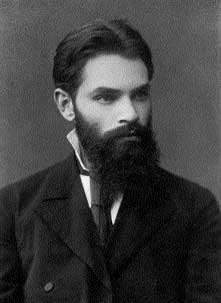
\includegraphics{dynamic/figures/a_lyapunov}
\caption{Aleksandr Lyapunov (1857–1918)}
\end{marginfigure}

Obviously, once the orbit moves away from $x_0$ to $x_1$, a first-order Taylor approximation around $x_0$ will probably no longer be very accurate, but we can play the same trick again, this time using an expansion around $x_1$. Starting from these observations, we can define some sort of average value of the derivative for the entire orbit. Conventionally, this is done using a geometric average, by defining the \textbf{Lyapunov number} of an orbit $\{x_0, x_1, x_2, ... \}$ as

\begin{equation}
\fbox{$\displaystyle
  L(x_0) = \lim _{n \to \infty}\left(\left|f'(x_0)\right|...\left|f'(x_{n-1})\right|\right)^{\frac{1}{n}}
$}  
\end{equation} 

if this limit exists.

The \textbf{Lyapunov exponent} is defined as the logarithm of the Lyapunov number:

\begin{equation}
h(x_0) = \ln L(x_0) = \lim _{n \to \infty}\frac{1}{n}\left(\ln\left|f'(x_0)\right| + ... + \ln\left|f'(x_{n-1)})\right|\right)
\end{equation} 

Note that $h$ exists if and only if $L$ exists and is non--zero.

E.g., if the Lyapunov number of an orbit is equal to 2, this means that on average the distance between the orbit of $x_0$ and a neighbouring orbit will double each iteration.

\begin{cue}
Which values of the Lyapunov number / Lyapunov exponent will correspond to chaos?  
\end{cue}

An orbit is called a \textbf{chaotic orbit} if its Lyapunov number is greater than 1 (or its Lyapunov exponent is positive). 

\pagebreak

\begin{exer}
% difficulty: hard  
The Lyapunov number of the orbit of $x_0$ under $f$ is $L$. What is the Lyapunov number of the orbit of $x_0$ under $f^k$? Also explain in words why this is plausible.
\end{exer}

\begin{exer}
% difficulty: normal  
Write a computer program to calculate the Lyapunov exponents for the family of logistic maps $f_a(x)=ax(1-x)$. Plot the Lyapunov exponent as a function of $a$. In which regions do you see chaos?
\end{exer}


\begin{exer}
% difficulty: normal
% ugent  
% credits: Chaos - Alligood
Making use of $\cos 2x = 1- 2 \sin^2 x$, prove the following explicit formula for any orbit of the logistic map $f(x) = 4x(1-x)$:

$$x_n= \frac{1}{2} -\frac{1}{2} \cos(2^n\arccos(1-2x_0))$$

Is this a useful formula from a computational point of view?
\end{exer}


\pagebreak

\sectionugent{2D maps - the H\'{e}non map}

\begin{marginfigure}
% credits: CNRS
% url: https://images.math.cnrs.fr/Michel-Henon-et-le-systeme-de-Henon-Heiles.html?lang=fr

\includegraphics{dynamic/figures/m_henon}
\caption{Michel H\'{e}non (1931-2013)}
\end{marginfigure}

The H\'{e}non map is to two--dimensional systems what the logistic map is to one--dimensional systems. It is governed by simple--looking equations, yet already exhibits most of the rich dynamic behaviour seen in more complicated systems.

The version of the H\'{e}non map that we will study is

\begin{equation}
f(x,y) = (a-x^2+by, x)
\end{equation} 

Depending on the values of $a$ and $b$, we can get radically different behaviours.

For starters, set $a=1.28$ and $b=-0.3$. If we start with the initial condition $(x,y)=(0,0)$, a numerical analysis tells us that the orbit moves towards a period--2 sink.

\begin{figure}[H]
\centering
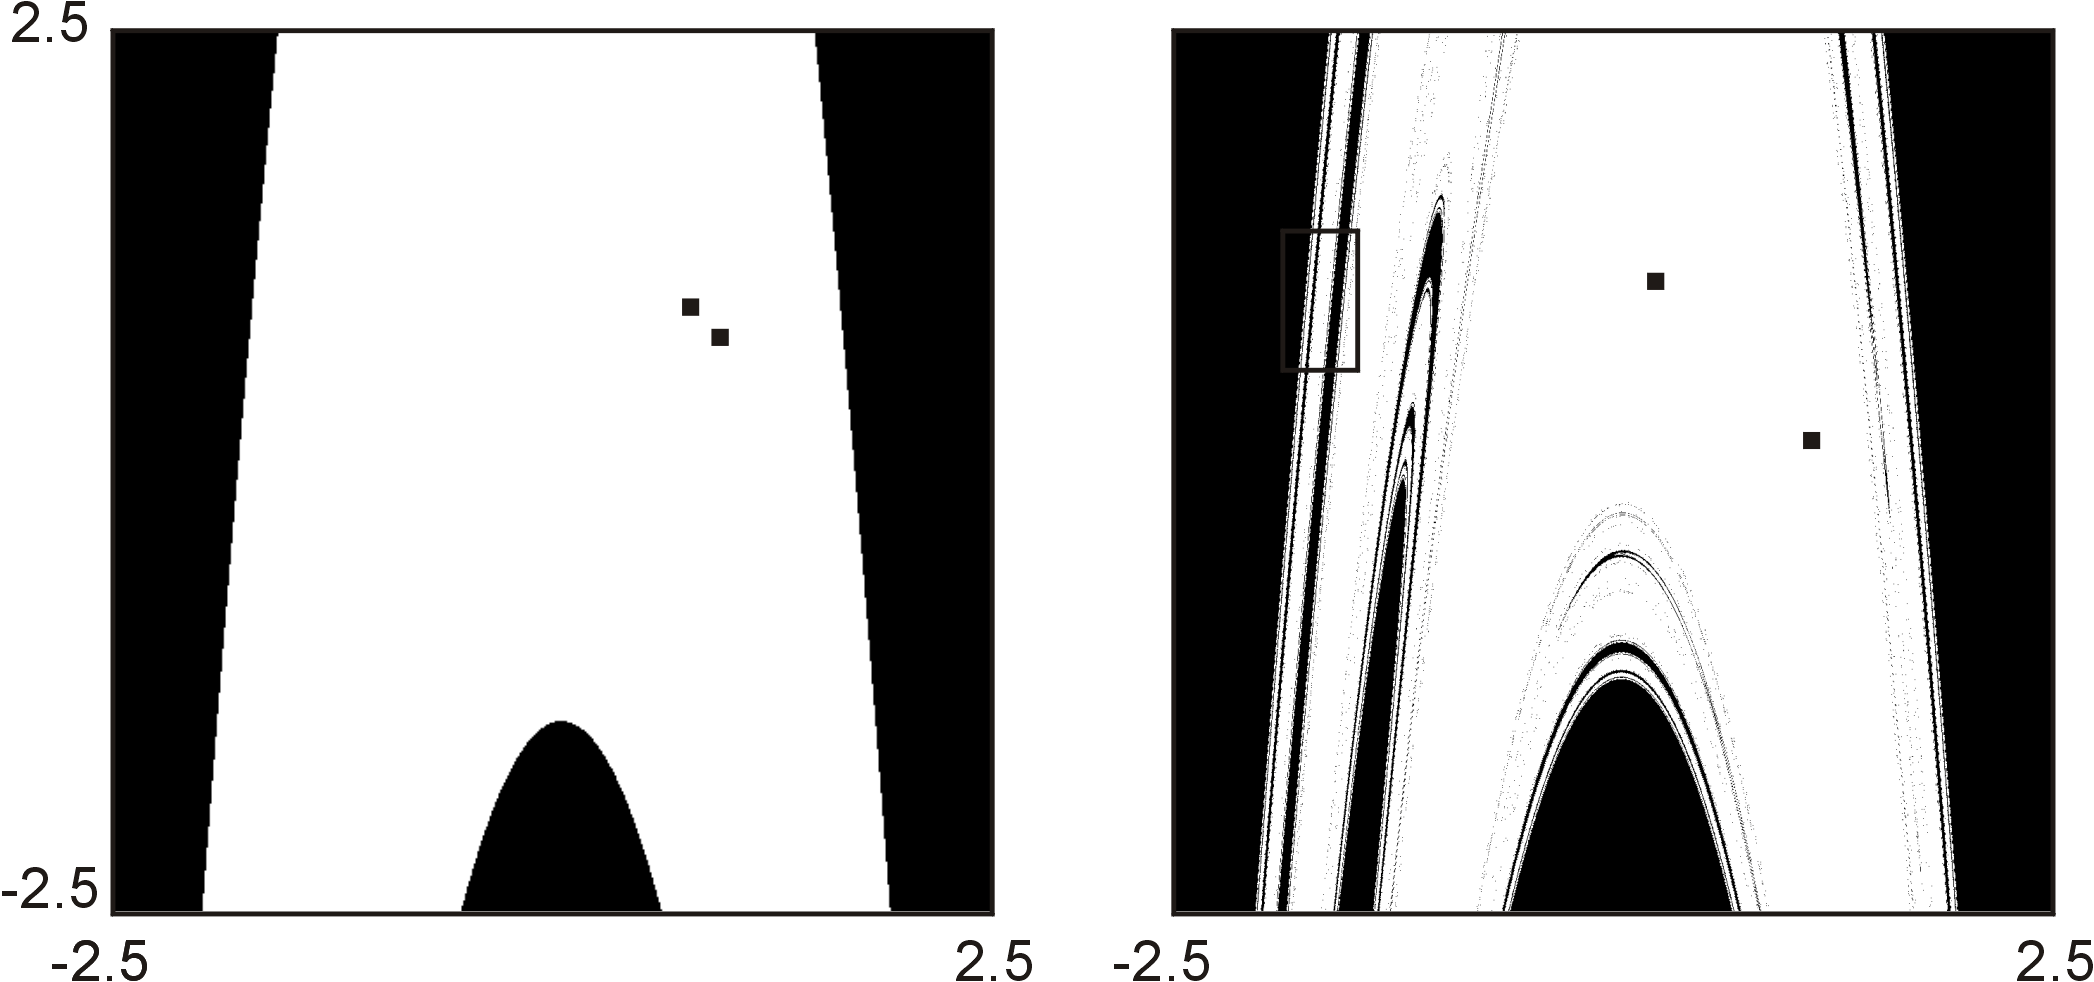
\includegraphics[width=11cm]{dynamic/figures/henon_basin}
\caption{Influence of initial conditions for the H\'{e}non map with $b=-0.3$. Initial values whose trajectories diverge to infinity are coloured black. The squares show a period--2 sink, which attracts white initial conditions. On the left, $a=1.28$ and the basin boundary is smooth. On the right, $a=1.4$, and the boundary is fractal.}
\label{fig-henon-basin}
\end{figure} 

The left part of Fig.~\ref{fig-henon-basin} shows an analysis of the results of iteration with general initial values. Points in black represent initial conditions whose orbits diverge towards infinity, white points are initial conditions which converge to the period--2 sink. For $a=1.28$ the boundary of the basin, which moves in and out of the rectangle of initial values shown here, is smooth.

For $a=1.4$ and $b=-0.3$, we get a completely different picture: the boundary of the basin is no longer smooth, but is in a sense infinitely complicated: if we were to zoom in on it, we would still see the same level of complexity, no matter how deep we would zoom. This is illustrated in Fig.~\ref{fig-henon-zoom}, which shows successive zooms of a small region of the basin boundary, indicated by a rectangle in the picture. \marginnote{Note that different zoom levels only need to look similar, not identical.}The \textbf{self--similarity} at different zoom levels is apparent. We call such a self--similar structure with infinite complexity a \textbf{fractal}.

\begin{figure}[H]
\centering
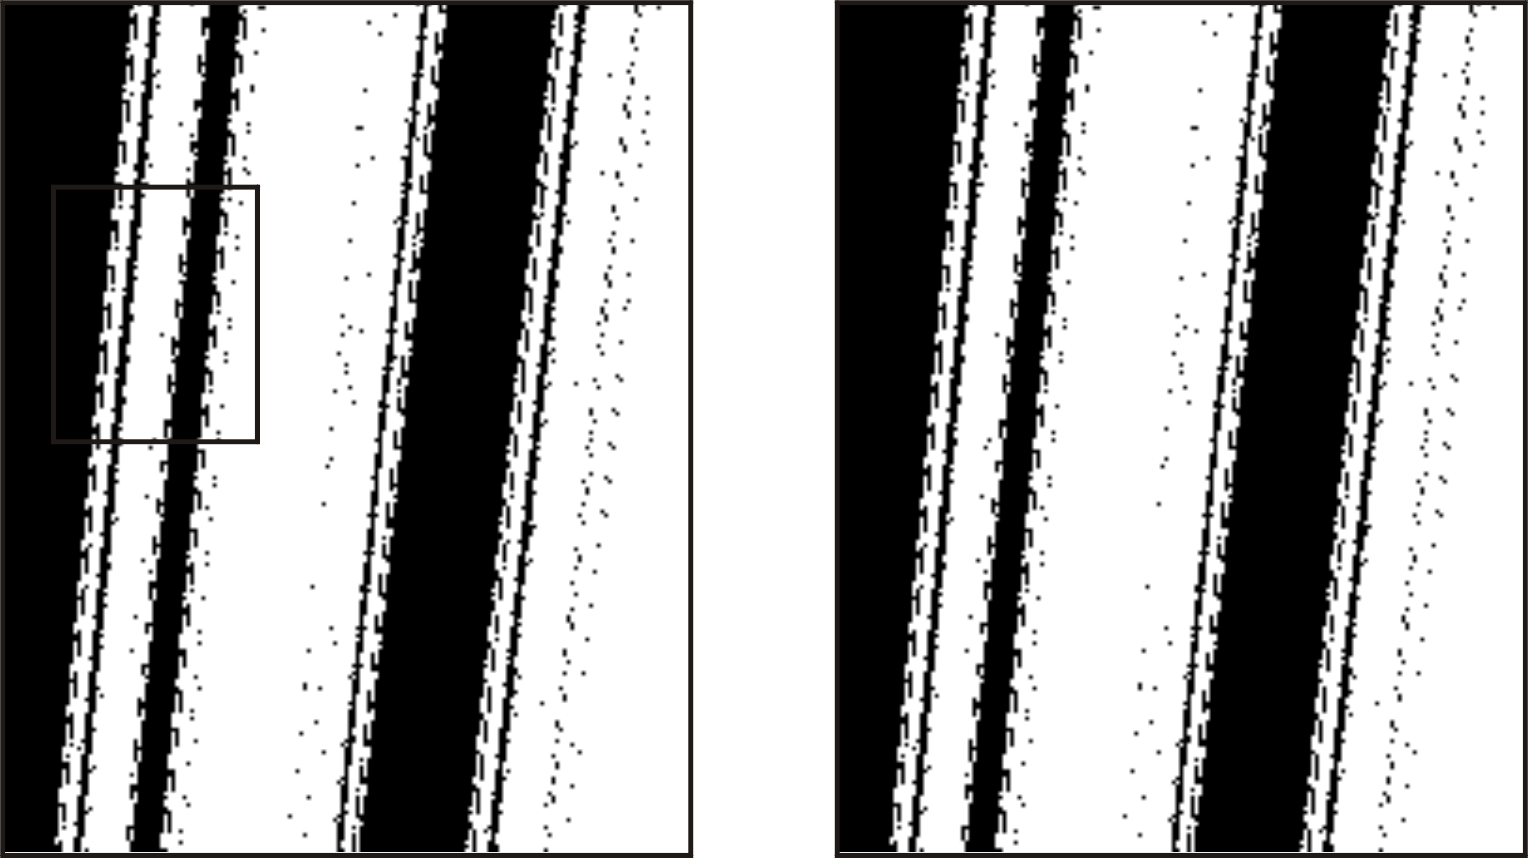
\includegraphics[width=8cm]{dynamic/figures/henon_zoom}
\caption{Self--similarity of the H\'{e}non basin boundary for $a=1.4$ and $b=-0.3$. The left picture corresponds to $[-1.88,-1.6] \times [-0.52,-0.24]$, which was indicated by the box in Fig.~~\ref{fig-henon-basin}. The right picture corresponds to the box in the left picture.}
\label{fig-henon-zoom}
\end{figure} 


\begin{marginfigure}
\centering
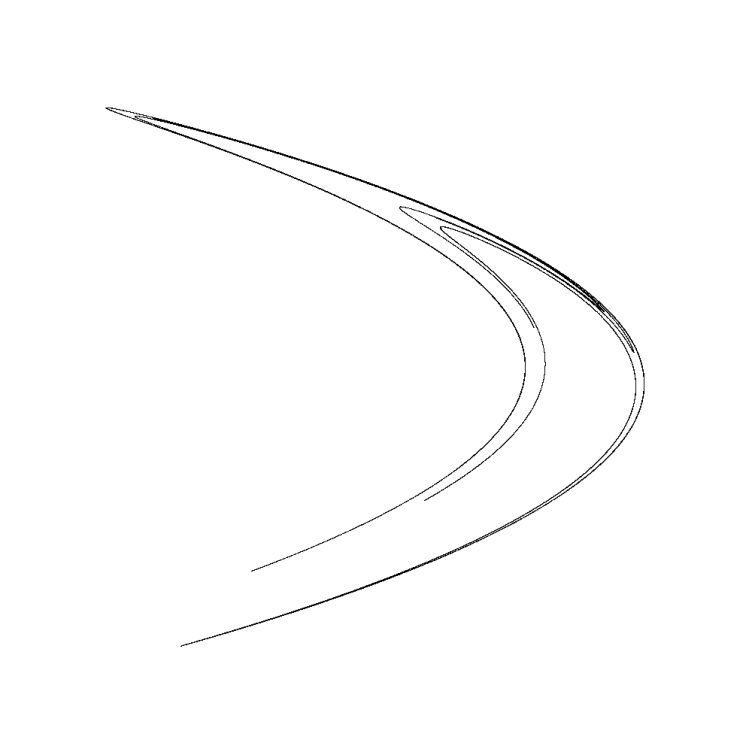
\includegraphics{dynamic/figures/henon_attractor}
\caption{Plot of the H\'{e}non attractor in the $(x,y)$--plane for $a=1.4$ and $b=0.3$.}
\label{fig-henon-attractor}
\end{marginfigure} 

Let us finally flip the sign of $b$ and look at the case $a=1.4$ and $b=0.3$. Now the period--2 sink disappears, and the orbit will eventually evolve to look like the structure in Fig.~\ref{fig-henon-attractor}. This is an example of a dynamical system with a \textbf{fractal attractor}, as it turns out that this attractor is once again self--similar at different zoom levels. The orbit of nearly any point in this region will converge to this attractor. Note that this does not mean that two slightly different initial conditions will converge to the same limiting behaviour. In fact, the opposite is true: because of the infinitely complicated nature of the attractor, the two orbits will eventually diverge and become completely uncorrelated.

\begin{cue}
Is there an orbit that continuously traces the attractor?  
\end{cue}

In a similar vein, don't get fooled by the continuous nature of the attractor. This does not mean that an orbit will just continuously trace out the attractor. This is nonsense, because we are working with discrete maps here. Rather, what will happen is that the orbit will 'jump' from one part of the attractor to another one, but all these individual points will eventually make up the continuous attractor.

\begin{exer}
% difficulty: trivial
Can you think of a self-silimar structure that appears in nature?
\end{exer}

\pagebreak

\begin{exer}
% difficulty: hard
Consider the following family of 2D maps, this time expressed in terms of a complex coordinate $z$:
$$P_c(z)=z^2+c$$
For each value of $c$, check numerically if the orbit of the initial point $z=0$ diverges towards infinity. Plot the points $c$ for which this orbit stays bounded. The set of these points is called the \textbf{Mandelbrot set}. By associating different colours for different speeds with which points run away towards infinity, you can also produce full-color versions of this picture.
\end{exer}

\begin{marginfigure}[2cm]
% credits: Wikipedia
% url: https://en.wikipedia.org/wiki/Benoit_Mandelbrot#/media/File:Benoit_Mandelbrot,_TED_2010.jpg
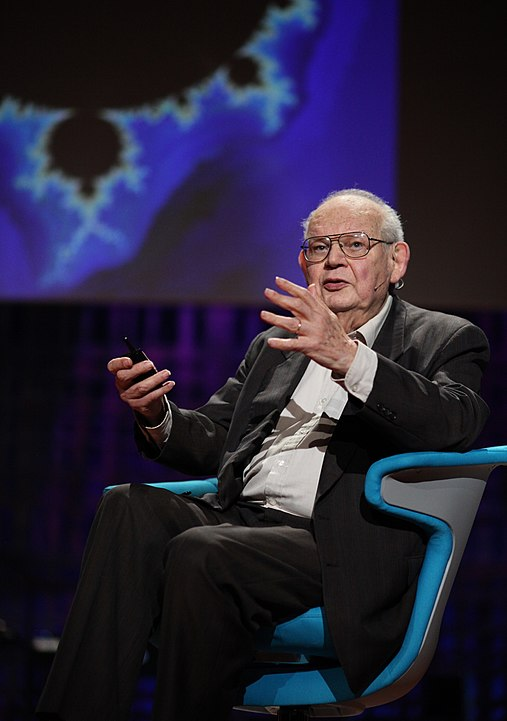
\includegraphics{dynamic/figures/b_mandelbrot}
\caption{Benoit Mandelbrot (1924-2010)}
\end{marginfigure}

\begin{figure}
\centering
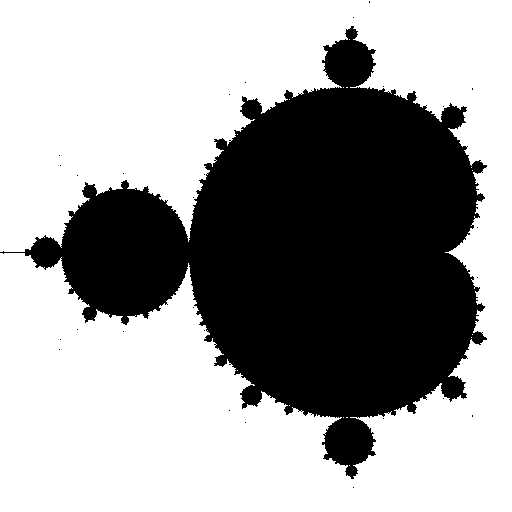
\includegraphics[width=7cm]{dynamic/figures/mandelbrot}
\label{fig-mandelbrot}
\end{figure} 


\begin{exer}
% difficulty: normal
Show that the Mandelbrot set has mirror symmetry along the real axis.
\end{exer}

\pagebreak

\sectionugent{Saddle points}

We used the term 'sink' in our discussion of 1D maps to refer to a fixed point or a periodic orbit that attracts an epsilon neighbourhood of initial values. A 'source' is a fixed point that repels a neighbourhood. These definitions make sense in higher--dimensional state spaces without alteration. In 2D e.g., the neighbourhoods in question are disks.

\begin{cue}
What would an image under the map of a disk around a sink or a source look like?  
\end{cue}

Fig.~\ref{fig-circle-images} shows schematic views of a sink and a source for a 2D map, together with a typical disk neighbourhood and its image under the map. Along with the sink and the source, a new type of fixed point is introduced, which cannot occur in 1D systems. This type of point, which we call a \textbf{saddle}, has at least one attracting direction and one repelling direction.

\begin{figure}[h]
\centering
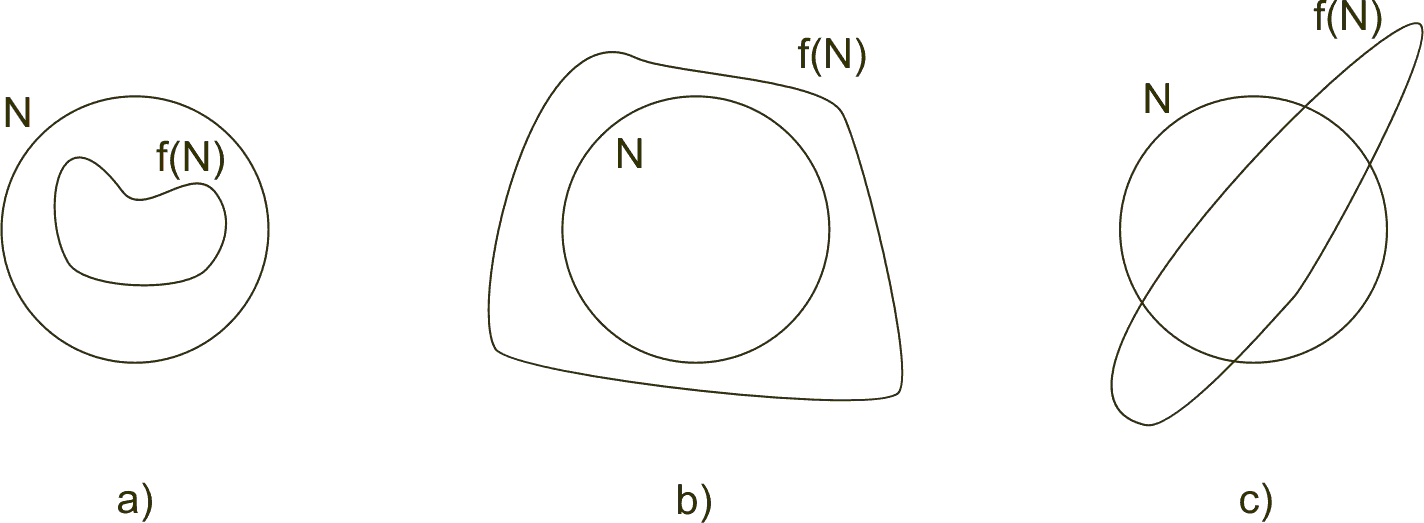
\includegraphics{dynamic/figures/circle_images}
\caption{Images of a disk $N$ in the neighbourhood of a $a)$ sink, $b)$ source, $c)$ saddle point.}
\label{fig-circle-images}
\end{figure} 

Points near this type of fixed point act as if they were moving along the surface of a cowboy's saddle under the influence of gravity. This is illustrated in Fig.~\ref{fig-saddle}.

\begin{cue}
Would you have sensitive dependence on initial conditions in the neigbourhood of a saddle?
\end{cue}

A saddle exhibits sensitive dependence on initial conditions, because of the neighbouring initial conditions that escape along the repelling direction.

\begin{marginfigure}
\centering
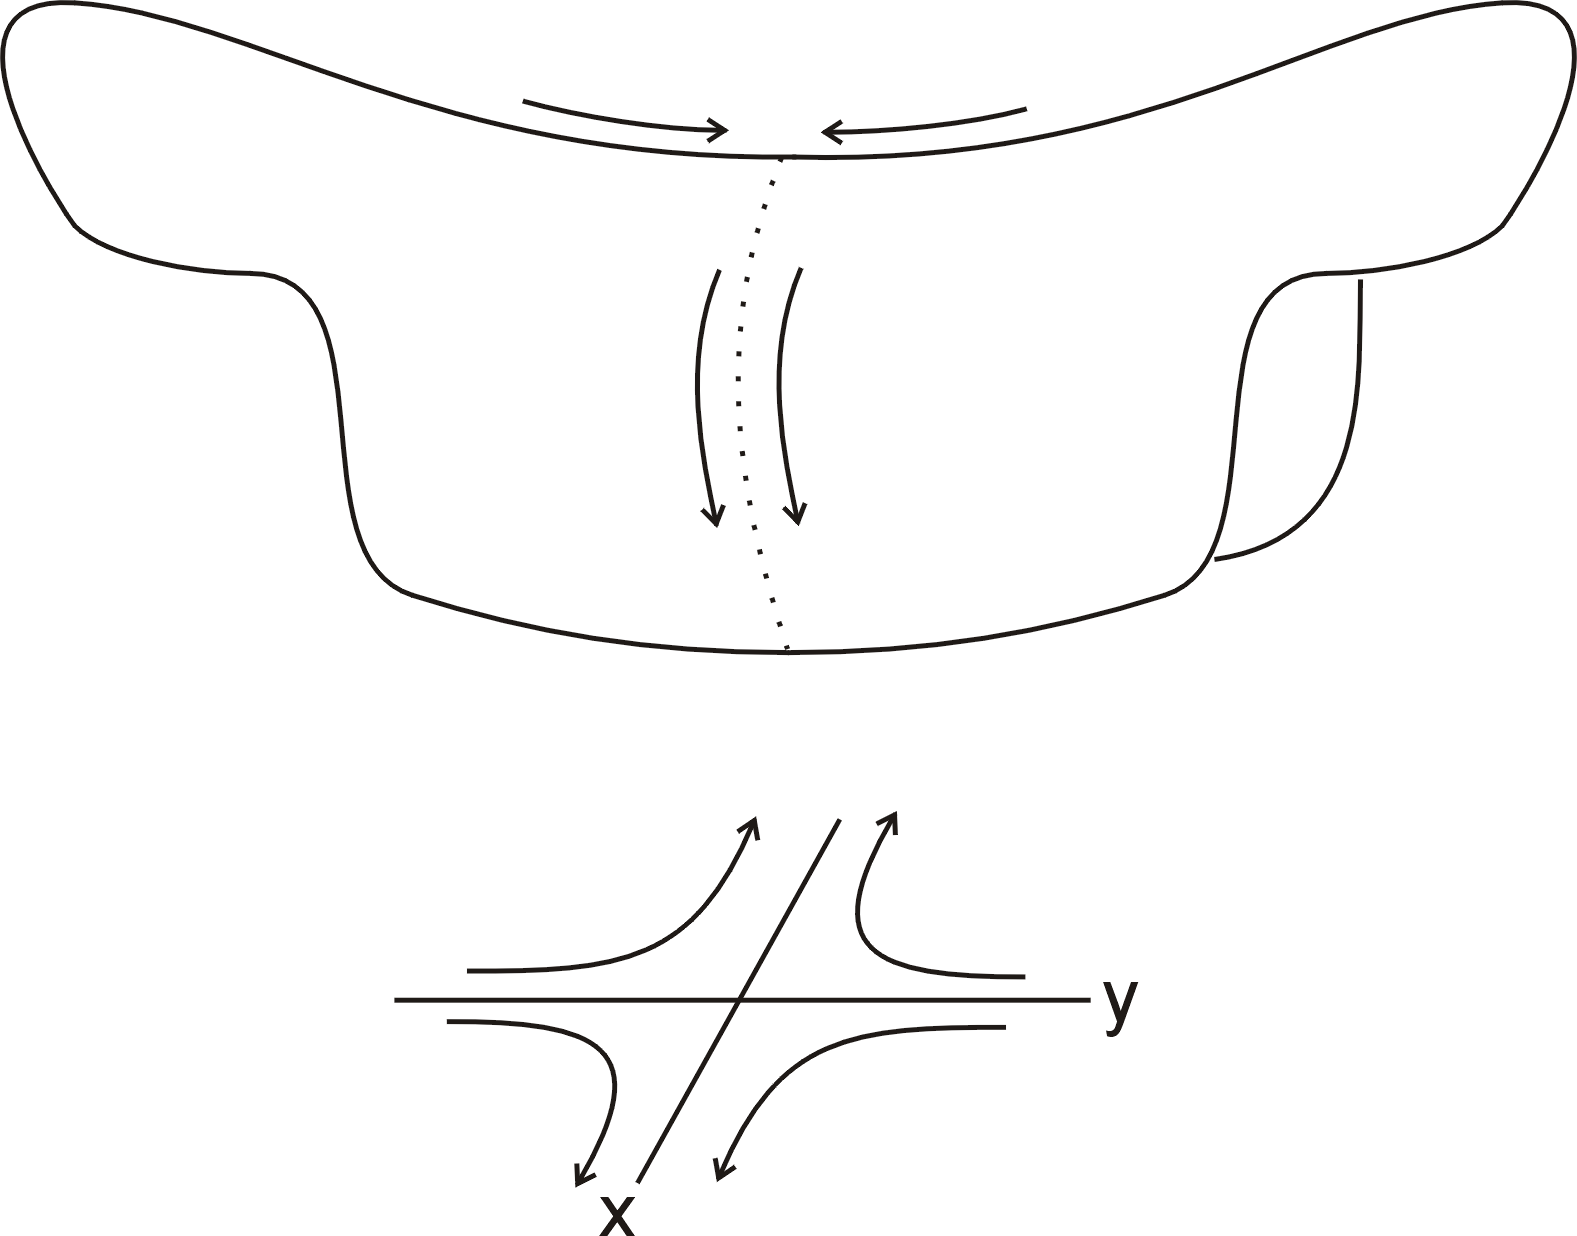
\includegraphics{dynamic/figures/saddle}
\caption{A saddle point.}
\label{fig-saddle}
\end{marginfigure} 

Saddle points play surprising roles in the dynamics of a system. To already give an example of this, let's return to Fig.~\ref{fig-henon-basin}, where black points are in the basin of infinity and white points are in the basin of sink. What happens to points which are located on the boundary between these two basins? Will they converge towards the sink or towards infinity? The answer is: neither. It turns out that these points converge towards the saddle! So, although not a general attractor, the saddle obviously plays an important role in determining which points go to which basin.

Our goal in the next sections is to find ways of identifying sources, sinks and saddles from the defining equations of the map. In 1D systems, we already saw that the key to determining stability was looking at the derivative in that point. Since the derivative determines the tangent line, or the best linear approximation near that point, it determines the amount of shrinking/stretching in the vicinity of that point. The same principle operates in higher dimensional systems, where we need to look at the best linear approximation of the system at that point. Before constructing such a linearisation, let's first study linear maps and see what we can learn from them.

\pagebreak

\sectionugent{Linear maps}

A 2D linear map is described by a simple matrix multiplication:

\begin{gather}
f(x,y) = {\mathbf A} 
\begin{bmatrix}
x \\
y
\end{bmatrix}
=
\begin{bmatrix}
a_{11} & a_{12} \\
a_{21} & a_{22}
\end{bmatrix}
\begin{bmatrix}
x \\
y
\end{bmatrix}
\end{gather} 

\begin{cue}
What is the fixed point of this map? In general terms, how would you study its stability? 
\end{cue}

Every linear map has a fixed point at the origin. Its stability can be investigated in the same way as we did for 1D maps: if all points in the neighbourhood of the fixed point approach the fixed point when iterated by the map, we consider the fixed point to be an attractor.

In some cases, the dynamics of a 2D system resemble 1D dynamics.

\begin{cue}
What does an orbit of an eigenvector of the map look like?  
\end{cue}

When the initial point ${\mathbf v_0}$ is an eigenvector of ${\mathbf A}$ with eigenvalue $\lambda$, we get:

\begin{gather}
{\mathbf v_1} = {\mathbf A}{\mathbf v_0} = \lambda {\mathbf v_0} \\
{\mathbf v_2} = {\mathbf A}\lambda {\mathbf v_0} = \lambda^2 {\mathbf v_0} 
\end{gather} 

and in general ${\mathbf v_n} = \lambda^n {\mathbf v_0}$. Hence the map behaves like the 1D map $v_{n+1} = \lambda v_n$.

The importance of eigenvalues is further exemplified by looking at the orbit of an arbitrary point. Let's restrict ourselves for the moment to the case where the eigenvalues $\lambda_i$ of ${\mathbf A}$ are distinct, so that we can diagonalise the matrix as follows (see your undergraduate linear algebra course):

\begin{equation}
{\mathbf A} = {\mathbf Q}
\begin{bmatrix}
\lambda_{1} & 0 \\
0 & \lambda_{2}
\end{bmatrix} 
{\mathbf Q^{-1}}
\end{equation} 

Here $\mathbf Q$ is a matrix whose columns are the eigenvectors of ${\mathbf A}$. 

\begin{cue}
Using this representation, calculate the orbit of an arbitrary point.
\end{cue}

After $n$ iterations, the orbit of a starting vector ${\mathbf x}_0$ looks as follows:

\begin{equation}
{\mathbf x}_n = {\mathbf A}^n {\mathbf x}_0 = {\mathbf Q}
\begin{bmatrix}
\lambda_1^n & 0 \\
0 & \lambda_2^n
\end{bmatrix} 
{\mathbf Q^{-1}} {\mathbf x}_0 
\end{equation} 

\begin{cue}
From this representation, what conclusions can you draw about the stability?  
\end{cue}

We see immediately that if all eigenvalues have a magnitude smaller than 1, the orbit converges to our fixed point $(0,0)$. On the other hand, if all eigenvalues have a magnitude larger than 1, the iterates will diverge, meaning that the fixed point is unstable. Finally, for one eigenvalue smaller than 1, and one eigenvalue larger than 1, we have saddle point, as there is one converging and one diverging direction.

\begin{exer}
% difficulty: normal 
  Not all $2 \times 2$ matrices can be diagonalised. We know from linear algebra that when the eigenvalues are not distinct, a canonical form is
  
\begin{equation}
{\mathbf A} = 
{\mathbf Q}^{-1}
\begin{bmatrix}
\lambda_1 & 1 \\
0 & \lambda_1
\end{bmatrix} 
{\mathbf Q}^{-1}
\end{equation} 

Show that in this case, the same conclusions with respect to stability of the fixed point hold as in the case of distinct eigenvalues.
\end{exer}


\begin{exer}
% difficulty: normal
% ugent
For the following maps, determine whether the origin is a sink, source or saddle.

a) $$\begin{bmatrix}4 & 30 \\ 1 & 3 \end{bmatrix}$$

b) $$\begin{bmatrix}1 & 1/2 \\ 1/4 & 3/4 \end{bmatrix}$$

\end{exer}


\begin{exer}
% difficulty: normal
% ugent  
Find

$$\lim_{n \to \infty}\begin{bmatrix}4.5 & 8 \\ -2 & -3.5 \end{bmatrix} ^ n \begin{bmatrix} 6 \\ 9 \end{bmatrix}$$

\end{exer}


\pagebreak

\sectionugent{Nonlinear maps and the Jacobian matrix}

Let's construct a linear approximation of an $N$-dimensional nonlinear map. To warm up, let's start with some simpler cases first.

\begin{cue}
Make a linear approximation of a 1D map, taking a single input $x$ to a single output $y$, for a point $p+h$ in the neighbourhood of a point $p$.  
\end{cue}

By truncating a Taylor series, we can write

\begin{equation}
f(p+h) - f(p) = \frac{df}{dx}(p)h + \mathcal{O}\left(|h|^2\right)
\end{equation} 

\begin{cue}
Now do the same for a function having $N$ inputs $x_1$, ... $x_N$ and a single output $y$.  
\end{cue}

For a function with multiple inputs, we get

\begin{equation}
  f(\mathbf{p}+\mathbf{h}) - f(\mathbf{p}) = \frac{\partial f}{\partial x_1}(\mathbf p)h_1+ \cdots +  \frac{\partial f}{\partial x_N}(\mathbf p)h_N+ \mathcal{O}\left(|\mathbf{h}|^2\right)
  \label{eq-multivar-approx}
\end{equation} 

In the equations above $\mathbf p$ and $\mathbf h$ are obviously $N$--dimensional vectors.

\begin{cue}
Finally, look at a vector function $\mathbf f$, i.e. a collection of $N$ functions $f_1(x_1, \cdots, x_N)$, ... , $f_N(x_1, \cdots, x_N)$. Why are we restricting ourselves to the case of the same dimension for the input and the output?
\end{cue}

Since we are looking at maps here, the dimension of the output has to be the same as the dimension of the input. By arranging $N$ versions of Eq.~\ref{eq-multivar-approx} in matrix form, we get

\begin{equation}
{\mathbf f}({\mathbf p} + {\mathbf h}) - {\mathbf f}({\mathbf p}) = \begin{bmatrix}
\frac{\partial f_1}{\partial x_1}({\mathbf p}) & \cdots & \frac{\partial f_1}{\partial x_N}({\mathbf p}) \\
\vdots & & \vdots \\
\frac{\partial f_N}{\partial x_1}({\mathbf p}) & \cdots & \frac{\partial f_N}{\partial x_N}({\mathbf p}) \\
\end{bmatrix} \cdot {\mathbf h} + \mathcal{O}\left(|{\mathbf h}|^2\right)
  \label{eq-jacobian}
\end{equation}


\begin{marginfigure}[-5.7cm]
  % credits: Wikipedia
  % url: https://en.wikipedia.org/wiki/Carl_Gustav_Jacob_Jacobi
  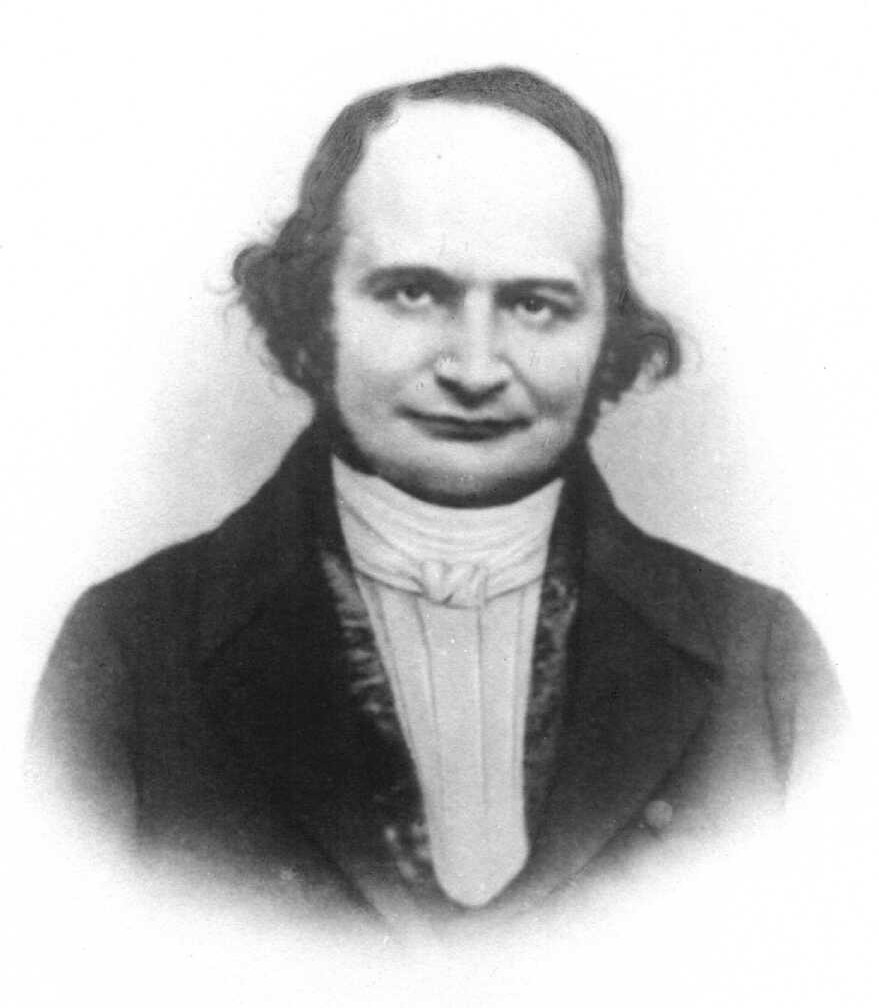
\includegraphics{numeric/figures/c_jacobi}
  \caption{Carl Gustav Jacob Jacobi (1804-1851)}
\end{marginfigure}

The matrix in Eq.~\ref{eq-multivar-approx} is called the \textbf{Jacobian}. We denote the Jacobian matrix of ${\mathbf f}$ at ${\mathbf p}$ as ${\mathbf Df}({\mathbf p})$.

So, given a vector ${\mathbf p}$ and a small increment ${\mathbf h}$, the increment in ${\mathbf f}$ due to ${\mathbf h}$ is given by

\begin{equation}
{\mathbf f}({\mathbf p} + {\mathbf h}) - {\mathbf f}({\mathbf p}) = {\mathbf Df}({\mathbf p}) \cdot {\mathbf h} + \mathcal{O}\left(|{\mathbf h}|^2\right)
\end{equation} 

\begin{cue}
If $\mathbf p$ is a fixed point of the nonlinear map $\mathbf f$, what happens to the distance $\mathbf h$ after applying the map?
\end{cue}

Our map takes $\mathbf p$ to $\mathbf p$ and ${\mathbf p} + {\mathbf h}$ to approximately $\mathbf p + {\mathbf Df}({\mathbf p}) \cdot {\mathbf h}$.

Looking only at the distances from $\mathbf p$, we can say that a distance $\mathbf h$  gets transformed to a distance  ${\mathbf Df}({\mathbf p}) \cdot {\mathbf h}$, which is a linear map in $\mathbf h$. 

As long as this distance remains small (so that $|{\mathbf h}|^2$ is negligible and our approximation is valid), the action of the nonlinear map $\mathbf f$ operating on inputs $\mathbf x$ near ${\mathbf p}$, is essentially the same as the linear map ${\mathbf A} = {\mathbf Df}({\mathbf p})$ operating on distances $\mathbf h$ near 0.

This map obviously has a fixed point ${\mathbf h} = 0$, and we can use our eigenvalue criteria for linear maps to study the stability of ${\mathbf Df}({\mathbf p})$. On the other hand, to draw conclusions about the associated non-linear map, although we won't prove it here, the following plausible stability criteria hold:

Let ${\mathbf f}$ be a map on $\mathbb{R}^n$ and assume ${\mathbf f}({\mathbf p})={\mathbf p}$.

\begin{enumerate}
\item
If the magnitude of each eigenvalue of ${\mathbf Df}({\mathbf p})$ is less than 1, then ${\mathbf p}$ is a sink of ${\mathbf f}$.
\item
If the magnitude of each eigenvalue of ${\mathbf Df}({\mathbf p})$ is greater than 1, then ${\mathbf p}$ is a source of ${\mathbf f}$.
\item
\noindent\marginnote{If none of the eigenvalues of ${\mathbf Df}({\mathbf p})$ are on the unit circle, $\mathbf p$ is called a \textbf{hyperbolic fixed point} of $f$.}If none of the eigenvalues of ${\mathbf Df}({\mathbf p})$ have magnitude equal to 1, if at least one eigenvalue of ${\mathbf Df}({\mathbf p})$ has magnitude less than 1, and at least one eigenvalue of ${\mathbf Df}({\mathbf p})$ has magnitude greater than 1, then ${\mathbf p}$ is a saddle of ${\mathbf f}$.
\end{enumerate}

\pagebreak

\begin{exer}
% difficulty: trivial
% ugent  
Consider the map 

$$f(x,y) = (-x^2+0.4y, x)$$

Discuss the stability of the fixed points $(0,0)$ and $(-0.6,-0.6)$.

\end{exer}

\begin{exer}
% difficulty: trivial 
% credits: Chaos - Alligood
Consider the map 

$$f(x,y) = (x^2-5x+y, x^2)$$

Find the fixed points and discuss their stability.
\end{exer}


\begin{exer}
% difficulty: hard  
Consider the linear map defined as $f(x,y) = (2x+y, x+y)$ with a corresponding matrix $A$. Discuss the stability of its fixed point.\\

Now, consider the nonlinear map defined as $g(x,y) = (2x+y, x+y)\, mod \, 1$, i.e. the same update rule as above but with an added modulo 1 operator. Show that $(1/3, 1/3)$ is a periodic point with period 4 of this nonlinear map.\\

Next, discuss the stability of this periodic point.\\

\textit{Hint}: the modulo operator can be applied after several updates and will lead to the same result, e.g.  $g(g(x,y)) = f(f(x,y)) \, mod \, 1$ (no need to prove this).\\
\textit{Hint 2}: consider $A^4 \begin{bmatrix} 1/3 + \delta_x \\ 1/3 + \delta_y \end{bmatrix} \, mod \, 1$ and looks what happens to the perturbation, without calculating any new eigenvalues, but using what you've determined about the stability of the fixed point of $A$.\\

Finally, you just showed that the point $(1/3, 1/3)$ is a periodic point, yet if we compute its evolution numerically we obtain a chaotic behaviour. Explain why.
\end{exer}


\pagebreak

\sectionugent{Stable and unstable manifolds}

Without providing any proofs, we will discuss in this section some more aspects of the special properties of saddle points.

We have seen that a saddle point is unstable, in the sense that most initial conditions will move away from it because the existence of an expanding direction. However, not all initial conditions will move away. Consider e.g. this very simple linear map:

\begin{equation}
A =
\begin{bmatrix}
0.9 & 0 \\
0 & 1.1
\end{bmatrix} 
\label{eq-map-ex}
\end{equation} 

\begin{cue}
What are the attracting and repelling directions of this map? Which points will converge to the saddle point? 
\end{cue}

For initial values on the $x$--axis, the orbit will converge to the saddle point, because it does not feel the influence of the expanding direction. This set of points is important enough to warrant its own name, for the case of general, nonlinear maps:

The \textbf{stable manifold} of a saddle point ${\mathbf p}$ is defined as the set of points ${\mathbf v}$ for which $|{\mathbf f}^n({\mathbf v}) - {\mathbf p} | \to 0$ as $ n \to \infty$.

\noindent\marginnote{A one--dimensional manifold is a set of points that locally looks like a line everywhere along its length. E.g. the letter 'O' is a 1--manifold. The letter 'T' on the other hand is not, because of the intersection and the end points.}For 2D maps, one can prove the following properties about the stable manifold. First of all, it is a one--dimensional manifold. Second, the stable manifold will be tangent to the eigenvector of the matrix ${\mathbf Df}({\mathbf p})$ with eigenvalue smaller than 1.

In the example from Eq.~\ref{eq-map-ex}, the $y$--axis is the \textbf{unstable manifold} of the saddle point.

\begin{cue}
How would you define an unstable manifold in general?  
\end{cue}

The unstable manifold of a saddle point ${\mathbf p}$ is defined as the set of points ${\mathbf v}$ for which $|{\mathbf f}^{-n}({\mathbf v}) - {\mathbf p}| \to 0$ as $ n \to \infty$, so points in the unstable manifold converge to the saddle point when iterating the map backwards. In other words, the unstable manifold is the stable manifold of the inverse map ${\mathbf f}^{-1}$.

Note that we have not defined the unstable manifold as the set of points for which $|{\mathbf f}^{n}({\mathbf v}) - {\mathbf p}| \to \infty$. Indeed, that would also include every point not on the stable manifold.

For the unstable manifold, similar properties hold as for the stable manifold. It is a 1D--manifold, and it is tangent to eigenvector of the Jacobian with eigenvalue larger than 1.

For linear maps, the stable and unstable manifolds are easily determined, and are just lines in the direction of the eigenvectors of the Jacobian. For nonlinear maps, they can look significantly more complicated, as is illustrated in Fig.~\ref{fig-manifold} for a H\'{e}non map. 

\begin{marginfigure}
\centering
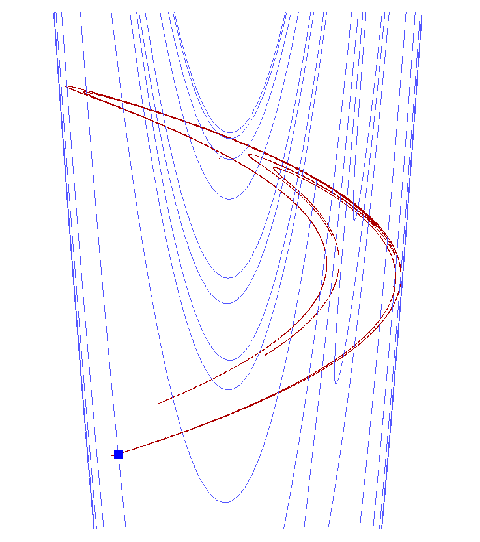
\includegraphics{dynamic/figures/manifold}
\caption{Stable and unstable manifold of a H\'{e}non map. The saddle point is the square in the lower left corner, the stable manifold is mainly vertical, the unstable one mainly horizontal.}
\label{fig-manifold}
\end{marginfigure} 

The shape of these curves should look familiar. Indeed, one can prove that the following properties hold:

\begin{enumerate}
\item
The stable manifold forms the boundary between the basin of the sink and the basin at infinity.
\item
The attractor of the map lies along the unstable manifold (which can be either a periodic sink, or a chaotic attractor)
\end{enumerate}

A further important aspect of the unstable and stable manifold is the following: if they cross (at another point than the saddle of course), there are automatically an infinite numbers of such crossings (which are called \textbf{heteroclinic points}). Also, the system will show chaotic behaviour in such a case.

These insights are mainly due to Poincar\'{e}, who developed much of the theory underlying chaotic systems when studying the dynamics of three bodies moving under the force of gravity.

\pagebreak

\sectionugent{Continuous systems}

In the last part of this chapter, we will discuss some introductory concepts on continuous dynamical systems, i.e. those that are described by differential equations rather than difference equations.

Since we have already spent so much time discussing discrete maps, it would be nice to have some tools to reduce a continuous system to a discrete one and be able to study some aspects of its dynamics in that way. There are two methods that can be used for this: the time--$T$ map and the Poincar\'{e} map.

A \textbf{time--$T$ map} is formed by taking snapshots at fixed time intervals of the solution of the continuous system, i.e. a time--$T$ map is a discrete map that advances the continuous system $T$ time units. 

Sometimes it is possible to write down an explicit equation for a time--$T$ map. Consider e.g. the differential equation which describes the cooling of an object with specific heat $k$:

\begin{equation}
\frac{dx}{dt} = -k x
\end{equation} 

Here $x$ stands for temperature.

\begin{cue}
Solve this equation and write down the corresponding time--$T$ map.  
\end{cue}

The solutions of this equation are of the form

\begin{equation}
x(t) = x_0 e^{-kt}
\end{equation} 

Advancing from time $t_0$ to $t_0+T$ amounts to a multiplication with $e^{-kT}$. So, the time--$T$ map for this system is the 1D map with the following update function:

\begin{equation}
f(x) = e^{-kT} x
\end{equation} 

If it's not possible to write down an explicit rule, then the map has to be iterated numerically.

Note that the laser dynamics example from the opening of the chapter also used the time--$T$ philosophy, as the system was studied at specific snapshots in time determined by the sampling frequency.

\begin{marginfigure}[-8.0cm]
  % credits: Wikipedia
  % url: https://en.wikipedia.org/wiki/Henri_Poincar%C3%A9#/media/File:PSM_V82_D416_Henri_Poincare.png
  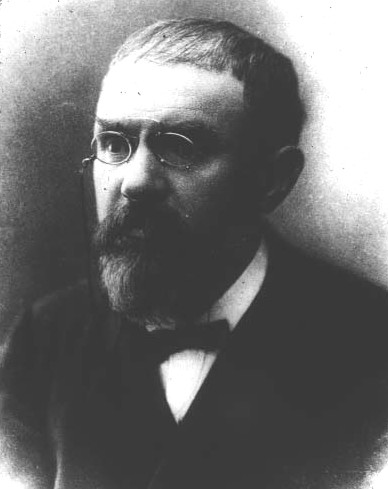
\includegraphics{dynamic/figures/poincare_photo}
  \caption{Henri Poincaré (1854-1912)}
\end{marginfigure}

Another technique to reduce a continuous system to a discrete one is the so--called \textbf{Poincar\'{e} map}. One of Poincar\'{e}'s most important innovations was a simplified way of looking at complex continuous trajectories. Instead of studying the entire trajectory, he found that much of the important information was encoded in the points at which the trajectory passes through a two--dimensional plane. The order of these intersection points defines a discrete plane map, which is called the Poincar\'{e} map. 

\begin{marginfigure}
\centering
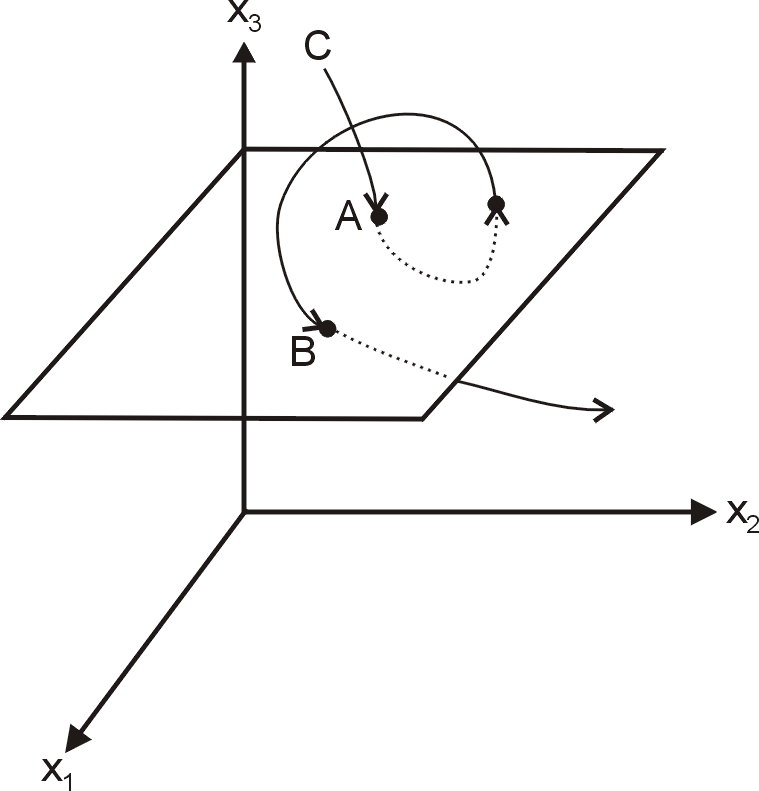
\includegraphics{dynamic/figures/poincare}
\caption{Poincar\'{e} map of a trajectory.}
\label{fig-poincare}
\end{marginfigure}

Fig.~\ref{fig-poincare} shows a schematic view of a trajectory $C$. The plane $S$ is defined by $x_3=$ constant. Each time the trajectory $C$ pierces $S$ in a downward direction, as at points ${\mathbf A}$ and ${\mathbf B}$, we record the point of piercing on the plane $S$. We can label these points with coordinates $(x_1,x_2)$. Let ${\mathbf A}$ represent the $k$--th downward piercing of the plane, and ${\mathbf B}$ the $(k+1)$--th downward piercing. The Poincar\'{e} map is the 2D map $G$ such that $G({\mathbf A}) = {\mathbf B}$.

Given ${\mathbf A}$, the differential equations can be solved with ${\mathbf A}$ as initial condition, and the solution followed until the next downward piercing at ${\mathbf B}$. Thus ${\mathbf A}$ uniquely determines ${\mathbf B}$, which ensures that the map $G$ is well--defined. Much of the dynamical behaviour of the trajectory $C$ is present in the 2D map $G$. E.g, if $C$ is periodic in the sense that it follows a closed loop, then the plane map $G$ will have a periodic orbit.

\begin{cue}
How are Poincar\'{e} maps and time--$T$ maps similar? How are they different?   
\end{cue}

The Poincar\'{e} map is similar in principle to the time--$T$ map we considered above, although the details are different. While the time--$T$ map is stroboscopic (it logs the value of a variable at equal time intervals), the Poincar\'{e} map records plane piercings, which need not be equally spaced in time.

\pagebreak

\sectionugent{Phase portraits}

If we do want to study the trajectory $C$ without reducing it to a discrete map, it is often useful to construct phase portraits (also called phase planes) of the solutions of a differential equation. 

To illustrate what these are, let's return to the simple differential equation

\begin{equation}
\frac{dx}{dt} = -k x
\end{equation} 

with solutions

\begin{equation}
x(t) = x_0 e^{-kt}
\end{equation} 

\begin{cue}
Plot a few of these trajectories for different starting points.  
\end{cue}

\begin{marginfigure}
\centering
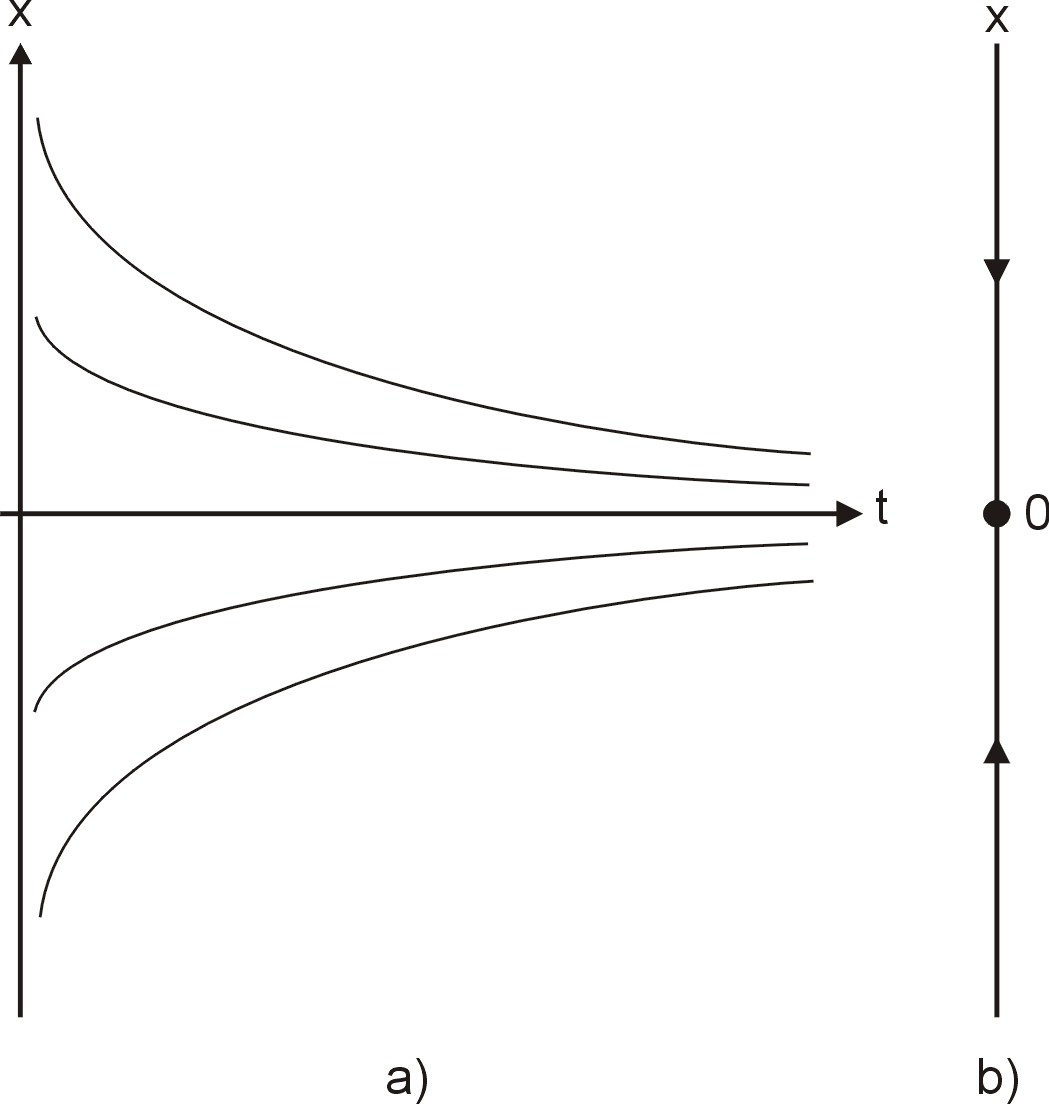
\includegraphics{dynamic/figures/phaseportrait}
\caption{$a)$ Solutions of ${dx}/{dt} = -k x$ for different initial conditions. $b)$ Corresponding phase portrait.}
\label{fig-phaseportrait}
\end{marginfigure} 

Fig.~\ref{fig-phaseportrait} a) sketches several trajectories of $x$ for different initial values. All curves converge to the equilibrium value $x=0$. An \textbf{equilibrium} solution is a solution of the differential equation which satisfies $dx/dt = 0$. They play the same role as fixed points in discrete maps, and are therefore important to study.

Often, a figure like Fig.~\ref{fig-phaseportrait}  a) contains too much information, as we are often only interested in the stability of the equilibrium. We are not so much interested in the different curves for different initial conditions, nor in the precise rate at which the equilibrium is approached. This leads to the \textbf{phase portrait} in Fig.~\ref{fig-phaseportrait} b), in which the $t$--axis is suppressed, and it is simply shown on the $x$--axis where trajectories are headed. The arrows indicate the direction of solutions (towards or away from equilibria) without graphing specific values of $t$. The phase portrait allows one to see at a glance where the equilibria are located and whether they are stable or not.


\begin{exer}
% difficulty: trivial  
Construct a phase portrait for the logistic differential equation:
$$\frac{dx}{dt} = a x (1-x)$$
\end{exer}

\pagebreak

\sectionugent{Example: the Lorenz attractor}

\begin{marginfigure}[0.0cm]
  % credits: Wikipedia
  % url: https://en.wikipedia.org/wiki/Edward_Norton_Lorenz#/media/File:Edward_lorenz.jpg
  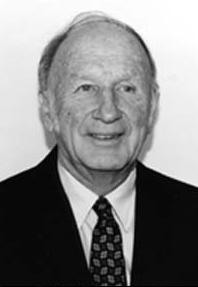
\includegraphics{dynamic/figures/e_lorenz}
  \caption{Edward Norton Lorenz (1917-2008)}
\end{marginfigure}

We finish the chapter by looking at the most famous set of differential equations which exhibit chaotic behaviour. They were formulated in the early 1960s by Lorenz, in the context of weather forecasting:

\begin{align}
\frac{dx}{dt} =& \, -\sigma x + \sigma y \\
\frac{dy}{dt} =& \, -xz + r y - y \\
\frac{dz}{dt} =& \, xy - bz
\end{align} 

For $\sigma=10$ and $b=8/3$, Lorenz found that the system behaves 'chaotically' whenever $r$ exceeds the critical value of $24.74$. In that case, all solutions appear to be extremely sensitive to initial conditions, and almost all of them are apparently neither periodic solutions nor convergent to periodic solutions or equilibria. Instead, he found found one of the very first chaotic attractors, which is now called the Lorenz attractor. This attractor is plotted in Fig.~\ref{fig-lorenz}.

\begin{marginfigure}
\centering
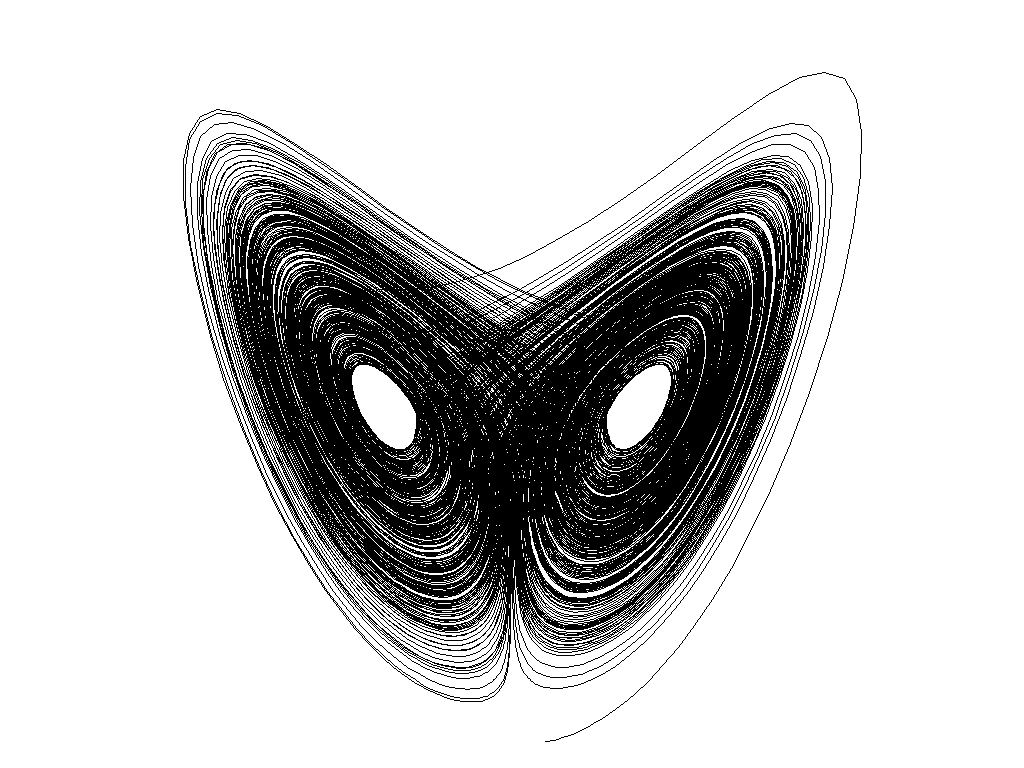
\includegraphics{dynamic/figures/lorenz}
\caption{The Lorenz attractor.}
\label{fig-lorenz}
\end{marginfigure} 


Lorenz realised that this sensitivity on initial conditions has a huge impact on weather predicting. In fact, the title of one of his talks was: "Predictability: Does the Flap of a Butterfly's Wings in Brazil set off a Tornado in Texas?". This is why sensitivity on initial conditions is sometimes referred to as 'the butterfly effect'.

\pagebreak

\section*{Review questions}

\begin{itemize}
\item What is a dynamical system? What types of dynamical systems are there?
\item What is an orbit?
\item How do you draw cobweb plots?
\item What are fixed points?
\item How do you investigate the stability of a fixed point?
\item What is the basin of a fixed point?
\item What are period points?
\item What is a bifurcation diagram?
\item What is chaos?
\item What is the Lyapunov number/exponent?
\item What is a self-similar/fractal structure? 
\item What is a fractal attractor?
\item What are saddle points?
\item How do you linearise a map? 
\item How do you investigate the stability of an $N$-dimensional nonlinear map? 
\item What is a 1D manifold in the geometric sense?
\item What are the stable and unstable manifolds of a saddle point?
\item What is a time-$T$ map?
\item What is a Poincar\'{e} map?
\item What is a phase portrait?
\item What are iconic examples of a 1D discrete map, a 2D discrete map and a continuous map?
\end{itemize}



%%% Local Variables:
%%% mode: latex
%%% TeX-master: "../main"
%%% End:
